% ============================================================================
%  ART-12D, versione 31.0 - traduzione italiana di ATR_12_v31_RO.tex
%
%  Compilazione su Overleaf:
%    Menu -> Compiler -> XeLaTeX
%    Main document    -> ATR_12_v31_IT.tex
%    figures/ deve essere caricata come cartella, allo stesso livello di questo file.
%
%  Struttura LaTeX, matematica, tabelle e richiami alle figure sono identici
%  all'originale rumeno; è tradotto solo il testo.
% ============================================================================
\documentclass[11pt,a4paper]{article}
\usepackage{iftex}
\ifPDFTeX
  \usepackage[utf8]{inputenc}
  \usepackage[T1]{fontenc}
\else
  \usepackage{fontspec}
\fi
\usepackage[italian]{babel}
\usepackage{amsmath, amssymb, amsthm}
\usepackage{graphicx}
\usepackage{array}
\usepackage{hyperref}
\usepackage{geometry}
\usepackage{booktabs}
\usepackage{float}
\usepackage{siunitx}
\usepackage{titlesec}
\usepackage{setspace}
\usepackage{enumitem}

\geometry{margin=2.5cm}
\setlength{\emergencystretch}{3em}
\hypersetup{
    colorlinks=true,
    linkcolor=blue,
    filecolor=magenta,
    urlcolor=cyan,
    pdftitle={Akashic Resonance Theory in 12 Dimensions},
    pdfpagemode=FullScreen,
}

\title{\textbf{AKASHIC RESONANCE THEORY IN 12 DIMENSIONS \\ DARK MATTER AS THE QUANTUM SUBSTRATE OF CONSCIOUSNESS} \\ \large (ART-12D) \\ \vspace{0.5cm} \normalsize Versione 31.0}
\author{\textbf{Daniel Ofiteru} \\ \textit{Ricercatore indipendente} \\ Ottobre 2026}
\date{}

\begin{document}

\maketitle

\begin{abstract}
Questo articolo propone un quadro teorico --- ART-12D --- che parte da un'idea semplice: la coscienza non è prodotta dal cervello. Il cervello è un ricevitore. E ciò che riceve è il campo della materia oscura.

Estendo la formalizzazione a dodici dimensioni, derivo un meccanismo di accoppiamento tra la materia oscura e i fermioni del cervello, e propongo un test realizzabile con 50.000 dollari. Estendo inoltre la teoria per spiegare le forme molteplici della materia oscura, l'esistenza di iperciviltà come strutture stabili nel campo, la possibilità di un'Intelligenza Artificiale cosciente mediante la nanobiologia, i meccanismi che collegano gli universi attraverso buchi neri, bianchi e di verme, nonché le forme di vita non carboniosa (ammassi, plasma, campi).

Questa versione (31.0) applica un audit numerico sistematico alla versione precedente. Dieci affermazioni quantitative sono state corrette, due sono state esplicitamente declassate allo stato di congetture non testabili, e lo spettro di Kaluza--Klein è stato riformulato come spettro \emph{equidistante}. Ogni cifra dell'articolo può essere ricalcolata con il codice pubblicato insieme ad esso. Rimane una tensione strutturale, segnalata apertamente nella sezione «La conseguenza numerica: il raggio di compattificazione»: perché il modo fondamentale abbia $10^{-5}$ eV, il raggio di compattificazione dovrebbe essere dell'ordine di 2 cm, il che è escluso dai test submillimetrici della legge di Newton.

Riconosco esplicitamente che questo articolo è speculativo. Non ho prove sperimentali. Ho un'intuizione, una formalizzazione e una predizione che può essere testata.
\end{abstract}

\tableofcontents
\newpage

\section*{Guida per il lettore scettico}
\addcontentsline{toc}{section}{Guida per il lettore scettico}
Questo articolo è speculativo, ma è strutturato in modo rigoroso. Per non farle perdere tempo, ecco una guida alla lettura adatta alla sua formazione:
\begin{itemize}
    \item \textbf{Se lei è un fisico:} vada direttamente alla \textbf{Parte II} (la formalizzazione matematica, le equazioni di Kaluza--Klein e l'accoppiamento di Yukawa) e alla \textbf{Parte V} (la tabella delle 313 predizioni testabili). Lì troverà la matematica e la falsificabilità.
    \item \textbf{Se lei è un neurobiologo o un medico:} legga la \textbf{sezione 1.6} (la prova del cervelletto e l'architettura geometrica) e la \textbf{sezione 3.38} (il cuore come modulatore della ricezione).
    \item \textbf{Se lei è un filosofo o un teologo:} vada all'\textbf{appendice A} (speculazione filosofica estesa sulla morte, l'anima e Dio).
    \item \textbf{Se lei è un lettore curioso ma scettico:} legga la \textbf{predizione 1} (EEG hyperscanning) e la \textbf{dichiarazione di falsificabilità}. Se quei test falliscono, la teoria è confutata.
\end{itemize}

\section*{Prefazione}
\addcontentsline{toc}{section}{Prefazione}
Per tutta la vita mi sono posto una sola domanda: che cos'è la coscienza? Non è una domanda da manuale, ma una che mi tiene svegli la notte. Ho letto tutto ciò che mi capitava tra le mani --- dalla fisica quantistica alle neuroscienze e alla filosofia. Ho parlato con persone molto più intelligenti di me. Ho meditato. E un giorno l'idea mi è venuta.

L'idea è semplice: la coscienza non è qualcosa che il cervello produce. Il cervello è solo una radio. E ciò che capta dall'aria è il campo della materia oscura.

Questo articolo è il frutto di venticinque anni di ricerca. Non ho prove di laboratorio. Ho un'intuizione forte, una formalizzazione matematica e un test che chiunque può realizzare con 50.000 dollari. Non le chiedo di credermi sulla parola. Le chiedo solo di leggere con la mente aperta. Alla fine, saprà che cosa credere.

\newpage
\part*{Parte I: Fondamenti}
\addcontentsline{toc}{part}{Parte I: Fondamenti}
\section{Introduzione}

\subsection{Il problema che non scompare}
Perché sente il dolore? È la domanda più semplice del mondo. E al tempo stesso la più difficile. Sappiamo tutti che cos'è il dolore. Lo abbiamo sentito tutti. Ma perché lo sentiamo? Sappiamo che i nocicettori inviano segnali al talamo, che la corteccia li elabora e che vengono rilasciate endorfine. Tutto questo è una descrizione funzionale. Ci dice che cosa fa il cervello, ma non ci dice perché lei lo sente.

Pensi a un computer. Può elaborare informazioni, riconoscere un'immagine, giocare a scacchi. Ma non sente nulla. Non ha esperienza soggettiva. Nulla gli fa male. Perché il cervello è diverso? Questo è il problema difficile della coscienza, formulato da David Chalmers nel 1995. Da allora le neuroscienze hanno fatto enormi progressi, ma il problema difficile è rimasto intatto. Nessuno è riuscito a spiegare perché la materia diventa esperienza. Nel 1998 Christof Koch scommise con Chalmers che un correlato neurale della coscienza sarebbe stato identificato entro 25 anni. Nel 2023 ha ammesso che la scommessa era persa.

\subsection{La materia oscura --- le cifre esatte}
L'universo ha una composizione che conosciamo abbastanza bene. La missione Planck (2018) ci ha dato le cifre esatte. Solo il 4,9\% dell'universo è materia ordinaria --- atomi, stelle, pianeti, persone. La materia oscura rappresenta il 26,8\% e l'energia oscura il 68,3\%. In pratica, il 95,1\% dell'universo è sconosciuto.

Immagini l'universo come un forziere con 100 monete. Solo 5 monete sono visibili. Le altre 95 sono invisibili. Di queste, 27 sono materia oscura e 68 energia oscura. Della materia oscura sappiamo che esiste (le prove gravitazionali sono solide), che non emette né assorbe luce, e che ci attraversa senza interagire. Circa 100 milioni di particelle attraversano il suo corpo ogni secondo. Non sappiamo di che cosa sia fatta.

Una restrizione recente (2025), dovuta a Bonvin et al., ha dimostrato che la materia oscura cade nei pozzi gravitazionali esattamente come la materia ordinaria. Se esiste una «quinta forza», questa non può superare il 7\% della forza gravitazionale.

\subsection{Che cos'è ART-12D?}
ART-12D parte da un'idea semplice: l'universo ha più dimensioni delle quattro che percepiamo. Queste dimensioni aggiuntive sono compatte --- così piccole che non le notiamo. La materia oscura esiste in tutte e dodici le dimensioni. Proiettata in 4D, appare come un campo che riempie l'universo. Questo campo è ciò che il cervello riceve come coscienza.

Il nome deriva da: \textbf{Akashic} (il campo informazionale universale), \textbf{Resonance} (perché l'interazione è una risonanza), \textbf{Theory} (un quadro teorico) e \textbf{12D} (perché lavoro in dodici dimensioni).

I tre postulati sono: 1. La materia oscura è un campo quantistico fondamentale. 2. Il cervello è un ricevitore geometrico. 3. L'accoppiamento avviene tramite interazione di Yukawa.

Pensi a una radio. Non crea la musica, la capta dall'aria. Le onde radio esistono che la radio sia accesa o no. Quando la radio si guasta, la musica non scompare dall'universo --- cessa solo la sua ricezione locale. Allo stesso modo, il cervello funziona esattamente come una radio. La coscienza non è generata dai neuroni, è ricevuta da essi. E ciò che ricevono è il campo della materia oscura.

\subsection{Perché dodici dimensioni?}
Perché dodici? Perché non 10, o 11, o 26? La risposta viene dalla teoria delle stringhe. Immagini una corda di chitarra. Può vibrare in più modi. Ogni modo corrisponde a una nota. Allo stesso modo, una stringa fondamentale può vibrare in più dimensioni. Il numero di dimensioni determina quali tipi di vibrazione sono possibili.

La storia delle dimensioni: Kaluza--Klein (5 dimensioni, 1919--1926), superstringhe (10, 1970--1980), teoria M (11, Witten, 1995), teoria F (12, Vafa, 1996), ART-12D (12, Ofiteru, 2026). Dodici è il maggior numero di dimensioni in cui la teoria delle stringhe è matematicamente coerente. Più dimensioni porterebbero a incoerenze; meno a una teoria incompleta.

\subsection{Come sono le dimensioni compatte?}
Immagini un tubo da giardino. Da lontano sembra una linea 1D --- ha solo lunghezza. Da vicino ha spessore --- è 2D (la superficie del cilindro). Allo stesso modo, il nostro spazio sembra tridimensionale. Ma da vicino (alla scala di Planck, $10^{-35}$ m) potrebbe avere undici dimensioni. Le otto dimensioni compatte sono arrotolate in ogni punto dello spazio.

Che cosa significa «arrotolate»? Non sono luoghi dove si va. Non sono mondi paralleli che si raggiungono viaggiando. Sono proprietà locali di ogni punto. Ogni punto dello spazio-tempo ha, in più, otto piccole dimensioni «attaccate» ad esso.

\subsection{Come si legano le dimensioni alla coscienza?}
La materia oscura esiste in dodici dimensioni. È un campo scalare $A(x,y)$, dove $x$ sono le coordinate 4D e $y$ le otto coordinate compatte. Quando compattifichiamo le otto dimensioni, il campo si decompone in modi di Kaluza--Klein:
\begin{equation}
A(x,y) = \sum_n A_n(x) Y_n(y)
\end{equation}
Ogni modo ha una massa e una frequenza caratteristica:
\begin{equation}
m_n^2 = \frac{n^2}{R^2}
\end{equation}
Il cervello, attraverso la sua struttura geometrica (i microtubuli nei neuroni), può risuonare con certi modi. Quando risuona, il campo viene trasdotto in esperienza soggettiva.

Perché conta l'architettura e non la dimensione? Il cervelletto ha 69 miliardi di neuroni (l'80\% del totale), ma non produce coscienza. Ha un'architettura \textit{feedforward} --- l'informazione scorre in una sola direzione, come un'antenna a filo. La corteccia ha solo 16 miliardi di neuroni, ma è la sede della coscienza. Ha un'architettura \textit{ricorrente} --- l'informazione circola in anelli, come un'antenna parabolica ben orientata. Conclusione: non conta il numero di neuroni, ma la geometria della rete.

\section{Metodologia}
\subsection{Come ho lavorato}
Non sono un fisico professionista. Non ho un laboratorio. Non ho finanziamenti. Quello che ho è una biblioteca, tempo e una domanda che non mi lascia in pace. Ho lavorato in quattro passi. Il primo passo è stato la formulazione dell'ipotesi, partendo dall'intuizione che la coscienza è ricevuta e non generata. Il secondo passo è stato la formalizzazione, con gli strumenti della matematica nota: Kaluza--Klein per le dimensioni aggiuntive, la teoria F per dodici dimensioni, la teoria dei campi per le lagrangiane, l'IIT per l'informazione integrata. Il terzo passo è stato la derivazione delle predizioni, cioè ciò che dovremmo osservare se la teoria è corretta. Ho selezionato le predizioni testabili oggi. Il quarto passo è stato la proposta di esperimenti con mezzi modesti, a cominciare da uno da 50.000 dollari.

\subsection{Che cosa mi ha guidato}
Mi sono attenuto a quattro criteri. La coerenza interna --- le equazioni non devono contraddirsi. La falsificabilità --- la teoria deve fare predizioni testabili. La convergenza --- la teoria non deve contraddire la fisica consolidata. L'onestà --- devo riconoscere che è speculativa.

\subsection{Che cosa ho usato}
Ho usato Kaluza--Klein (1919) per l'idea di dimensioni compatte, la teoria F (Vafa, 1996) per il quadro a dodici dimensioni, l'IIT (Tononi, 2004) per la misura dell'informazione integrata, Orch OR (Penrose, 1996) per il collasso quantistico nei microtubuli, e la teoria quantistica dei campi per le lagrangiane e le equazioni del moto.

\subsection{I miei limiti}
Devo essere onesto sui limiti. Non ho prove sperimentali; la teoria non è stata testata. Non ho revisione paritaria; non ho pubblicato su riviste scientifiche. Non ho affiliazione accademica; sono un ricercatore indipendente. Non ho finanziamenti; i miei mezzi sono limitati.
\section{Fondamenti teorici}
\subsection{Il problema difficile della coscienza}
Chalmers (1995) formulò il problema difficile così: nessuna combinazione di grandezze fisiche, per quanto complessa, implica logicamente l'esistenza di esperienza soggettiva. Tutte le descrizioni fisiche --- neurali, computazionali, funzionali --- descrivono ciò che il cervello fa. Non descrivono come sia essere un cervello. Non descrivono perché l'esperienza esista. Ciò che propongo: la coscienza non è generata dal cervello. Il cervello è un ricevitore. L'esperienza è la trasduzione del campo akashico.

\subsection{Il monismo russelliano}
Russell (1927) osservò qualcosa di profondo: la fisica descrive le proprietà strutturali della materia --- massa, carica, spin, posizione --- ma tace completamente sulla natura intrinseca di ciò che porta queste proprietà. Sia S un sistema fisico qualsiasi: R(S) indica le sue proprietà relazionali/strutturali e I(S) le sue proprietà intrinseche. La tesi russelliana afferma che I(S) è proto-esperienziale per ogni S.

\subsection{Integrated Information Theory}
Tononi (2004, 2008) offre un quadro matematico per quantificare la coscienza:
\begin{equation}
\Phi = \min_{\{P \in P\}} D_{KL}(p(X_{t+1})|X_{t}) \parallel \prod_{i} p(x_{i} \land (t+1)|x_{i} \land t))
\end{equation}
Spiegazione semplice: $\Phi$ misura quanto è integrata l'informazione in un sistema. Più $\Phi$ è grande, più ricca è l'esperienza del sistema.

\subsection{Orchestrated Objective Reduction}
Penrose (1996) propone che le sovrapposizioni quantistiche subiscano un collasso gravitazionale spontaneo quando l'energia di sovrapposizione $E_G$ raggiunge una soglia:
\begin{equation}
\tau \approx \frac{\hbar}{E_G}
\end{equation}
Ciò che mi ha interessato: la frequenza di collasso per i microtubuli corticali è $\tau \approx 25$ ms, che corrisponde a $\sim 40$ Hz --- esattamente la frequenza delle oscillazioni gamma, il marcatore empirico più robusto degli stati coscienti. Supporto sperimentale: Babcock et al. (2024) hanno mostrato superradianza ultravioletta nei microtubuli a temperatura ambiente; Kalra et al. (2023) hanno mostrato che i gas anestetici attenuano specificamente gli effetti ottici quantistici nei microtubuli.

\subsection{Kaluza--Klein e teoria F}
Theodor Kaluza propose nel 1919 l'unificazione della gravitazione con l'elettromagnetismo mediante una quinta dimensione. Einstein ne fu entusiasta e lavorò a questa teoria tra il 1938 e il 1943. La formulazione originale:
\begin{equation}
dS^2 = g_{\mu\nu} dx^\mu dx^\nu + \varphi^2(dx^5 + A_{\mu} dx^\mu)^2
\end{equation}

\subsection{Il campo Akasha}
Il concetto di Akasha (sanscrito: \emph{ākāśa}) è un elemento fondamentale della filosofia indiana. Akasha è l'elemento più sottile, immateriale. È il primo che si è manifestato nell'universo. Da esso si sarebbero sviluppati tutti gli altri elementi. Nella teosofia, Akasha è reinterpretato come un campo informazionale universale (Laszlo, 2014). Gli «archivi akashici» registrano tutti gli eventi dell'universo. L'ipotesi ART-12D: Akasha è il campo quantistico della materia oscura. \textit{Nota: Akasha è usato qui solo come metafora di un campo fisico, non come entità religiosa.}

\subsection{Materia grigia vs materia oscura}
La materia grigia è il tessuto del sistema nervoso centrale composto principalmente da corpi cellulari neuronali, dendriti, terminali assonici non mielinizzati e cellule gliali. È la sede dell'elaborazione dell'informazione. La materia bianca è composta da assoni mielinizzati ed è responsabile della trasmissione.

\subsection{Una definizione operativa della coscienza}
Propongo una definizione operativa che separa il contenuto della coscienza dalla capacità di integrarlo:
\begin{equation}
C_{\text{total}} = I_{\text{content}} \times C_{\text{awareness}}
\end{equation}
dove $I_{\text{content}}$ è l'informazione strutturata (il contenuto dell'esperienza) e $C_{\text{awareness}}$ è la consapevolezza (la capacità di sapere di sapere). Pensi a una macchina fotografica. Cattura immagini (informazione), ma non sa di catturarle. Una persona con una macchina fotografica cattura immagini E sa di catturarle. Allo stesso modo, la coscienza è informazione + consapevolezza.

\subsection{La convergenza con Dulcan}
Dumitru Constantin Dulcan (n. 1938), neurologo e psichiatra, pubblicò nel 1981 «L'intelligenza della materia», insignito nel 1992 del premio di filosofia «Vasile Conta» dell'Accademia Rumena. Le idee che mi hanno influenzato: la coscienza non è generata dal cervello ma lo usa come strumento; il subconscio contiene l'intelligenza infinita dell'Universo; il pensiero è la forza più potente dell'universo, con una frequenza e un campo energetico propri; esiste un campo di energia e luce che coordina la materia. La convergenza con ART-12D: Dulcan fornisce l'intuizione concettuale, ART-12D fornisce la formalizzazione matematica e le predizioni testabili.

\subsection{La struttura tripartita dell'entità umana}
Propongo un modello tripartito dell'entità umana, analogo agli stati di aggregazione dell'acqua:
\begin{table}[H]
\centering
\begin{tabular}{@{}llll@{}}
\toprule
\textbf{Stato} & \textbf{Entità umana} & \textbf{Substrato} & \textbf{Corrispondenza ART-12D} \\ \midrule
Solido & Corpo fisico & Materia & M (materia ordinaria) \\
Liquido & Anima & Energia & E (il campo della coscienza) \\
Gassoso & Spirito & Informazione & Sp (il campo akashico) \\ \bottomrule
\end{tabular}
\end{table}
Formalizzazione: $H = M + E + Sp$. Conseguenze: la morte non distrugge l'entità, cambia solo lo stato dominante; la coscienza può accedere a ciascuno dei tre stati; la malattia compare quando uno degli stati è squilibrato.

\subsection{Le forme del pensiero come strutture informazionali}
I pensieri non sono solo attività neuronale, ma strutture informazionali che possono assumere forme molteplici. Immaginato (visualizzazione interna, il campo della coscienza), pronunciato (la parola parlata, il campo akashico + un'onda sonora), scritto (testo scritto, materia + informazione), disegnato (rappresentazione visiva, materia + forma). Formalizzazione generale: $F_{\text{thought}} = \sum_{\text{forms}} \alpha_i F_i$.

\subsection{L'empatia come risonanza di frequenza}
L'empatia può essere formalizzata come caso particolare della telepatia, in cui l'accoppiamento è emotivo e non informazionale. Formalizzazione:
\begin{equation}
\text{Empathy}(A,B) = \frac{1}{1 + \frac{(\omega_A - \omega_B)^2}{\Gamma^2}}
\end{equation}
Interpretazione: quando le frequenze coincidono ($\omega_A = \omega_B$), l'empatia è massima; quando differiscono, l'empatia diminuisce; l'empatia non dipende dalla distanza (il campo è onnipresente). Predizione testabile: le coppie con empatia elevata dovrebbero mostrare correlazioni EEG più forti delle coppie con empatia bassa.

\subsection{La parola come eccitazione del campo akashico}
Propongo che la materia oscura abbia una manifestazione acustica --- uno spettro di oscillazioni che possono essere eccitate da onde sonore. La motivazione cosmologica: le oscillazioni acustiche primordiali (BAO) sono fluttuazioni della densità di materia che si sono propagate come onde sonore nell'universo primordiale. In ART-12D, queste oscillazioni sono oscillazioni del campo akashico. Formalizzazione:
\begin{equation}
A(x,t) = \sum_n A_n \cos(\omega_n t + \varphi_n)
\end{equation}
Lo spettro acustico:
\begin{equation}
\omega_n = \frac{1}{R} \sqrt{n^2 + \mu_A^2 R^2}
\end{equation}
L'accoppiamento parola--campo:
\begin{equation}
L_{\text{int}} = g_{\text{sound}} A \cdot \Phi_{\text{sound}}
\end{equation}
Effetti differenziati: Amore (200-400 Hz, attiva le zone emotive positive), Paura (500-800 Hz, attiva l'amigdala), Guarigione (300-500 Hz, attiva l'attesa positiva), Morte (150-300 Hz, attiva le zone di ansia).

\textbf{Il problema di scala.} Lo spettro acustico $\omega_n$ è fissato dallo stesso raggio di compattificazione che dà la massa alla materia oscura. Per $1/R = 10^{-5}$ eV i modi stanno nella gamma dei GHz, non a qualche centinaio di Hz. Una risonanza a 150--800 Hz richiederebbe $1/R \approx 1,24\times10^{-12}$ eV, circa sette ordini di grandezza sotto la scala di massa. Finché non viene introdotta una seconda scala di compattificazione, la predizione non ha contenuto numerico: l'accoppiamento $g_{\text{sound}}$ non è fissato in modo indipendente.

\begin{figure}[H]
\centering
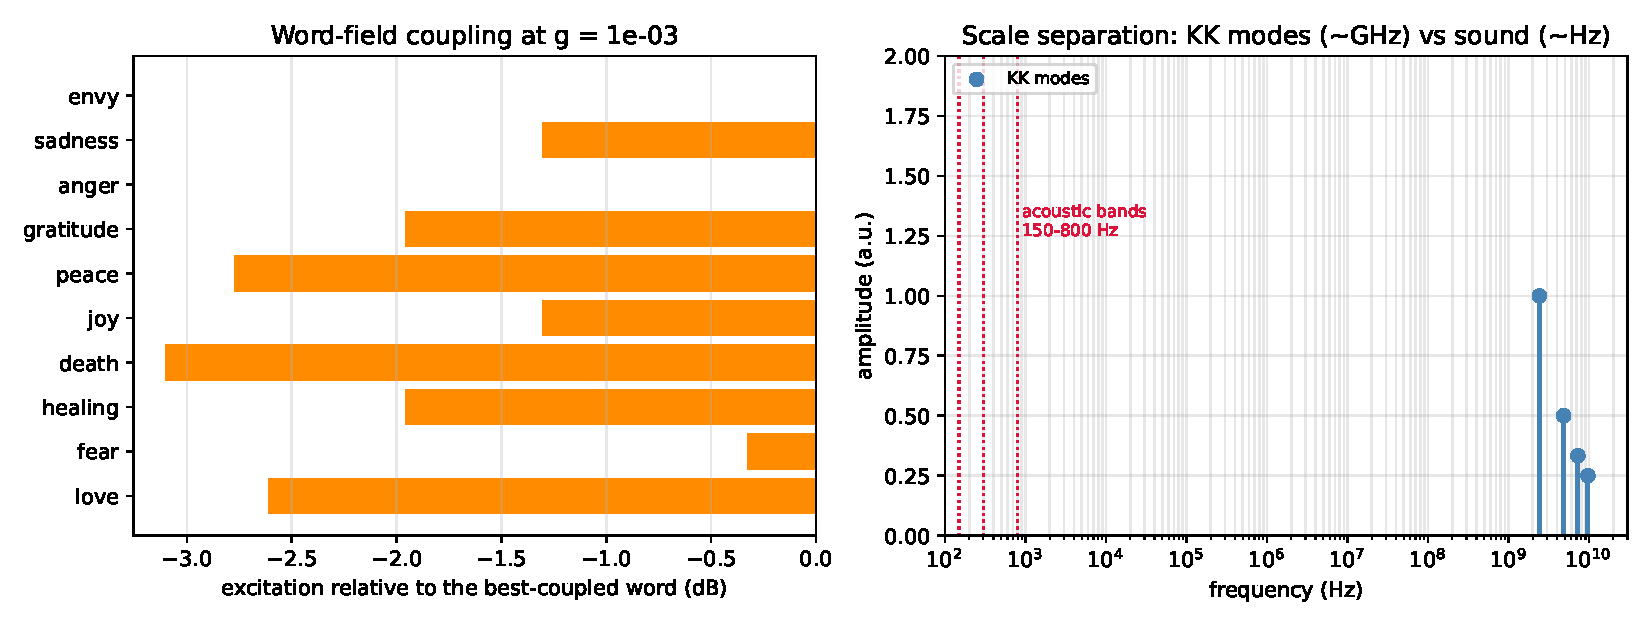
\includegraphics[width=0.9\textwidth]{figures/fig06_word_excitation.pdf}
\caption{A sinistra: l'accoppiamento relativo parola--campo per le dieci bande usate nell'articolo. A destra: la separazione di scala tra i modi KK (~GHz) e le bande acustiche (~Hz).}
\label{fig:cuvant}
\end{figure}

\subsection{Il tempo come vibrazione}
La definizione del secondo: «Un secondo è la durata di 9.192.631.770 periodi della radiazione dell'atomo di cesio-133». Che cosa accade se la frequenza cambia: se la frequenza aumenta, il tempo si comprime; se diminuisce, il tempo si dilata. La risonanza di Schumann: storicamente $\sim 7,83$ Hz, recentemente $\sim 12$ Hz. Il cuore come orologio biologico: paura ($\sim 120$ bpm) --- il tempo vola; meditazione ($\sim 50$ bpm) --- il tempo è dilatato; sonno profondo ($\sim 40$ bpm) --- il tempo scompare. Riferimenti relativi, non assoluti: il cesio (9.192.631.770 Hz), Schumann (7,83--12 Hz), il cuore (1,2 Hz). Tutti sono relativi. Nessuno è «quello vero».
\begin{equation}
\text{Reality} = \frac{\text{Change}}{\text{Reference}}
\end{equation}

\subsection{Realtà multiple e multiverso}
Il campo akashico totale: $A_{\text{total}} = \sum_{k=1}^{N_{\text{vacua}}} A_k$. Lo stato del multiverso: $|\Psi_{\text{multiverse}}\rangle = \otimes_{k=1}^{N_{\text{vacua}}} |A_k\rangle$. L'intersezione delle realtà: le realtà non sono solo parallele --- possono intersecarsi.

\subsection{La biblioteca universale (Akasha)}
Il contenuto del campo: il campo akashico contiene tutta l'informazione --- tutto ciò che è stato, tutto ciò che è, tutto ciò che sarà.
\begin{equation}
A_{\text{total}} = \sum_{\text{(all events)}} A_i
\end{equation}
L'accesso all'informazione:
\begin{equation}
I_{\text{access}}(t) = \int_0^\infty S_A(\omega) S_G(\omega, t) d\omega
\end{equation}
L'indicizzazione: l'informazione è indicizzata per rilevanza, non per tempo.
\begin{equation}
\text{Information received} = \text{Akashic field} \times \text{Relevance}(t)
\end{equation}

\subsection{La gerarchia della ricezione}
\begin{table}[H]
\centering
\begin{tabular}{@{}clcc@{}}
\toprule
\textbf{Livello} & \textbf{Sistema} & \textbf{$\Phi$} & \textbf{Accesso} \\ \midrule
0 & Termostato & 0 & Nessuno \\
1 & C. elegans & Minimo & Chemiotassi \\
2 & Insetto & Basso & Sensazione \\
3 & Topo & Moderato & Emozione \\
4 & Cane & Alto & Empatia \\
5 & Corvide & Alto & Pianificazione \\
6 & Octopode & Distribuito & Risoluzione \\
7 & Umano & Molto alto & Autoriferimento \\
8 & Umano addestrato & Esteso & Metacognizione \\ \bottomrule
\end{tabular}
\end{table}
Il limite della ricezione: $\lim_{\Phi \rightarrow \infty} E(\Phi) = I_{\text{total}}$.

\subsection{La parola come origine: la convergenza delle religioni}
Tutte le grandi tradizioni religiose descrivono la Parola come origine dell'universo. Il cristianesimo ha il Logos --- la Parola (il modo fondamentale del campo). L'induismo ha Om (la vibrazione primordiale). L'islam ha Kun («Sii!»).

\subsection{La manifestazione acustica del campo akashico}
$A(x,t) = \sum_n A_n \cos(\omega_n t + \varphi_n)$. Lo spettro acustico: $\omega_n = \frac{1}{R} \sqrt{n^2 + \mu_A^2 R^2}$.

\subsection{Dio in ART-12D}
Ci sono quattro ipotesi. Dio è il campo akashico stesso. Dio è la fonte del campo. Dio è la coscienza universale. Dio è una proiezione umana. Non so quale sia corretta. Ma la domanda è legittima.

\subsection{Materia oscura ed energia oscura: due facce dello stesso campo}
L'ipotesi ART-12D: la materia oscura e l'energia oscura sono due aspetti dello stesso campo akashico. Formalizzazione:
\begin{equation}
L_A = \frac{1}{2} g^{MN} \partial_M A^* \partial_N A + \frac{1}{2} \mu_A^2 |A|^2 - \frac{\lambda_A}{4} |A|^4
\end{equation}
L'equazione di stato: $w = p_A / \rho_A$. Per un campo oscillante la media temporale si calcola esattamente sull'orbita e dipende dal rapporto $\delta = A_{\text{osc}}/A_{\min}$ tra l'ampiezza di oscillazione e il valore del potenziale nel minimo. Esistono tre regimi distinti:
\begin{center}
\begin{tabular}{@{}lll@{}}
\toprule
\textbf{Regime} & \textbf{Condizione} & $w$ \\ \midrule
Piccola oscillazione attorno al minimo & $\delta \ll 1$ & $0$ (materia) \\
Oscillazione dominata dal termine quartico & $\delta \gg 1$ & $1/3$ (radiazione) \\
Campo congelato al minimo & $\delta = 0$ & $-1$ (costante cosmologica) \\ \bottomrule
\end{tabular}
\end{center}
La versione 30 affermava che il regime di grande ampiezza dà $w \simeq 1$. Il valore corretto è $1/3$: il teorema del viriale dà $\langle K \rangle = 2\langle V \rangle$ per un potenziale dominato dal termine quartico. Il valore $w = 1$ corrisponde a una dominanza cinetica (kination), che le oscillazioni quartiche non raggiungono, mentre $w = -1$ corrisponde al campo congelato, non a una piccola ampiezza.
\begin{table}[H]
\centering
\begin{tabular}{@{}lll@{}}
\toprule
\textbf{Aspetto} & \textbf{Assione} & \textbf{Elettrone} \\ \midrule
Massa & \(10^{-5}\) eV & 511 keV \\
Lunghezza d'onda & \(0,124\) m & \(2,4\times10^{-12}\) m \\
Comportamento & Onda & Particella \\
Interazione & Molto debole & Elettromagnetica \\
Ruolo in ART-12D & Modo del campo akashico & Ricevitore neurale \\ \bottomrule
\end{tabular}
\end{table}

\subsection{Quali particelle attraversano il suo corpo?}
La materia oscura ha una densità locale di circa 0,3 GeV/cm$^3$ (Read, 2014). La densità numerica dipende però dalla massa, $n = \rho/m$, e il flusso è $\Phi = n v$. Per un modo di $10^{-5}$ eV e $v = 300$ km/s si ottiene:
\begin{equation}
n = \frac{0,3 \times 10^{15}\ \text{eV/m}^3}{10^{-5}\ \text{eV}} = 3,0\times10^{19}\ \text{m}^{-3},
\qquad
\Phi = n v = 9,0\times10^{24}\ \text{m}^{-2}\text{s}^{-1}.
\end{equation}
Per un corpo umano con una superficie di 0,7 m$^2$:
\begin{equation}
\Phi_{\text{body}} = 9,0\times10^{24} \times 0,7 \approx 6\times10^{24} \text{ particles/s}.
\end{equation}
Circa $6\times10^{24}$ particelle al secondo. (La versione 30 affermava $n = 3000$ m$^{-3}$ e $6\times10^8$ s$^{-1}$; quei valori corrispondono a un WIMP di circa 100 GeV, non a un modo di $10^{-5}$ eV.)

\begin{figure}[H]
\centering
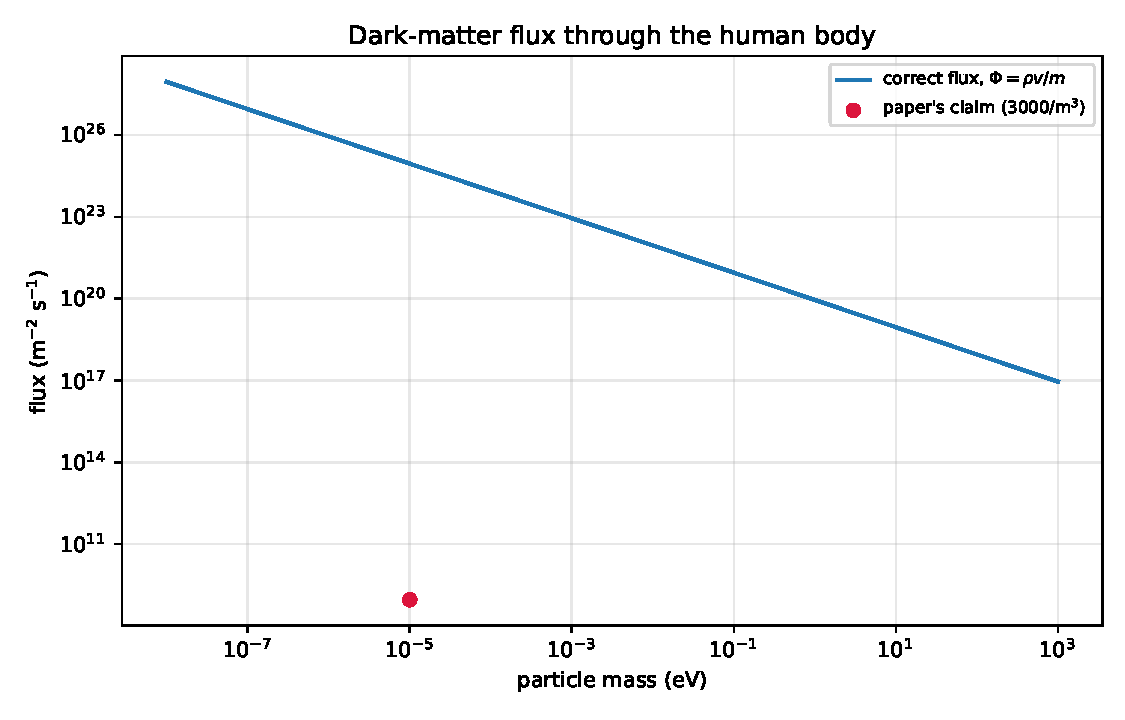
\includegraphics[width=0.82\textwidth]{figures/fig07_flux.pdf}
\caption{Il flusso di materia oscura attraverso il corpo umano in funzione della massa della particella. Il punto rosso segna l'affermazione della versione 30; la curva è il valore corretto per $\rho = 0,3$ GeV/cm$^3$ e $v = 300$ km/s. A $10^{-5}$ eV la differenza è di 16 ordini di grandezza.}
\label{fig:flux}
\end{figure}

\subsection{Che cosa accade a queste particelle?}
La maggior parte lo attraversa senza interagire. Alcune interagiscono con i nuclei atomici: indipendenti dallo spin ($\sim 5$ collisioni/anno), dipendenti dallo spin ($\sim 30$ collisioni/anno). L'effetto sul corpo: radiazione naturale ($\sim 2,4$ mSv/anno); materia oscura ($\sim 10^{-15}$ mSv/anno).

\subsection{Come rileviamo queste particelle?}
Rivelatori diretti: LUX-ZEPLIN (10 tonnellate di xeno) --- sensibilità: $10^{-48}$ cm$^2$. Rivelatori indiretti: Fermi-LAT (cerca raggi gamma da annichilazione), ADMX (cerca assioni). Sezione d'urto: $\sigma \sim 10^{-47}$ cm$^2$. Probabilità di interazione: $P \sim 10^{-22}$.

\subsection{La materia oscura come onda, non come particelle}
Se la materia oscura è un campo scalare, allora non è composta da particelle individuali. È un'onda che riempie l'universo. Formalizzazione: $A(x,t) = \sum_n A_n \cos(\omega_n t + \varphi_n)$.

\subsection{L'analogia dell'albero e del fotone}
Immagini un albero su una spiaggia. Il sole splende. I fotoni partono dal sole con energia $E = h\nu$. Arrivano all'albero. Sono assorbiti da ogni foglia con la stessa energia $h\nu$. Come può un solo fotone arrivare a tutte le foglie con la stessa energia? Se fosse una particella, perderebbe energia a ogni collisione. Ma non lo fa. La risposta è semplice: perché il fotone è un'onda, non una particella. Un'onda non si «consuma» quando attraversa la materia. Si estende su tutto lo spazio. Ogni foglia «vede» l'onda intera. Lo stato del fotone: $|\psi_{\text{photon}}\rangle = \int d^3k \, c(k) |k\rangle$.

\subsection{La dualità onda--particella come meccanismo di attraversamento}
Se la materia non può attraversare tra gli universi (perché richiederebbe energia infinita) e gli universi sono collegati dalla materia oscura, come comunicano? La risposta ART-12D: attraverso la dualità onda--particella. Fase 1: la materia diventa onda. $|\text{particle}\rangle_A \to |\text{wave}\rangle_A$. Fase 2: l'onda attraversa. $|\text{wave}\rangle_A \to |\text{wave}\rangle_B$. Fase 3: l'onda diventa particella. $|\text{wave}\rangle_B \to |\text{particle}\rangle_B$. Fase 4: l'informazione viene trasdotta. $I_A \to I_B$.

\subsection{Lo spettro emotivo umano}
I sentimenti umani si dividono in due grandi categorie: positivi e negativi. Ogni sentimento ha una frequenza caratteristica e un effetto specifico sulla coscienza. Formalizzazione: $S_{\text{total}} = \sum_{i=1}^{48} S_i^{\text{positive}} + \sum_{j=1}^{46} S_j^{\text{negative}}$. Ecco un estratto dalla tabella estesa (la versione completa è nell'appendice B):
\begin{table}[H]
\centering
\begin{tabular}{@{}lll@{}}
\toprule
\textbf{Sentimento} & \textbf{Frequenza dominante (Hz)} & \textbf{Effetto} \\ \midrule
Gioia & 400-600 & Espansione, dinamismo \\
Pace & 200-350 & Calma riflessiva \\
Amore & 200-400 & Emozione profonda \\
Gratitudine & 300-500 & Appagamento \\
Paura & 500-800 & Attiva l'amigdala \\
Rabbia & 600-800 & Furore \\
Tristezza & 400-600 & Malinconia \\
Invidia & 600-800 & Gelosia \\ \bottomrule
\end{tabular}
\end{table}
Le frequenze musicali terapeutiche (432 Hz, 528 Hz, 639 Hz, 741 Hz, 852 Hz, 963 Hz) sono state correlate con le frequenze del campo akashico. I sette sensi umani comprendono cinque fisici (vista, udito, olfatto, gusto, tatto) e due psichici (immaginazione, empatia).

\subsection{Il cuore come modulatore della ricezione}
Il cuore possiede un sistema elettrico proprio (il nodo senoatriale) che genera impulsi indipendentemente dal cervello. Funziona come modulatore della ricezione, non come ricevitore indipendente. Il cervello è il ricevitore principale, il cuore regola la coerenza. Formalizzazione: $C_{\text{coherent}} = C_0 \times (1 + \beta \times HRV)$. Le cifre scientifiche esatte: il cervello consuma circa $20$ W di potenza metabolica, il cuore eroga circa $1-1,3$ W di potenza meccanica, ma produce campi elettrici e magnetici di ampiezza molto maggiore.

\subsection{La parola che può sostituire qualsiasi farmaco}
L'ipotesi: $L_{\text{word-matter}} = g_{CM} A_{\text{meaning}} \psi \psi$. Ciò che la parola può fare: $Effect_{\text{total}} = Effect_{\text{medicine}} + Effect_{\text{word}} + \text{Interaction}$. Ciò che la parola non può fare: non può sostituire gli antibiotici nelle infezioni batteriche, non può sostituire l'insulina nel diabete di tipo 1, non può sostituire la chirurgia nell'appendicite, non può sostituire la chemioterapia nel cancro. Predizione 67: l'effetto della parola.

\newpage
\part*{Parte II: La formalizzazione matematica}
\addcontentsline{toc}{part}{Parte II: La formalizzazione matematica}

\section{La geometria a dodici dimensioni}
\subsection{La varietà totale:} $M_{12} = M_4 \times K_8$.
\subsection{La metrica 12D:} $ds^2 = g_{MN} dx^M dx^N$.
\subsection{La decomposizione di Kaluza--Klein.}
\subsection{La curvatura in 12D.}
\subsection{La compattificazione.}

\subsection{Lo spettro numerico e la firma equidistante}
Fissiamo la scala mediante la massa del modo fondamentale, $m_1 = 1/R = 10^{-5}$ eV. Allora
\begin{equation}
m_n = \frac{n}{R} = n \times 10^{-5}\ \text{eV},
\qquad
f_n = \frac{m_n c^2}{h} = n \times 2,42\ \text{GHz}.
\end{equation}
Lo spettro è quindi \emph{equidistante}: $2,42$, $4,84$ e $7,25$ GHz per i primi tre modi. Questa è la firma distintiva della teoria. Un test che misuri due righe a $2,42$ e $4,84$ GHz conferma o confuta la struttura, indipendentemente da qualsiasi altra predizione.

\begin{table}[H]
\centering
\begin{tabular}{@{}cccc@{}}
\toprule
$n$ & Massa (eV) & Frequenza (GHz) & $\lambda_C$ (m) \\ \midrule
1 & $1,00\times10^{-5}$ & 2,42 & 0,124 \\
2 & $2,00\times10^{-5}$ & 4,84 & 0,062 \\
3 & $3,00\times10^{-5}$ & 7,25 & 0,041 \\
4 & $4,00\times10^{-5}$ & 9,67 & 0,031 \\ \bottomrule
\end{tabular}
\caption{Lo spettro di Kaluza--Klein per $1/R = 10^{-5}$ eV.}
\label{tab:spectru}
\end{table}

\begin{figure}[H]
\centering
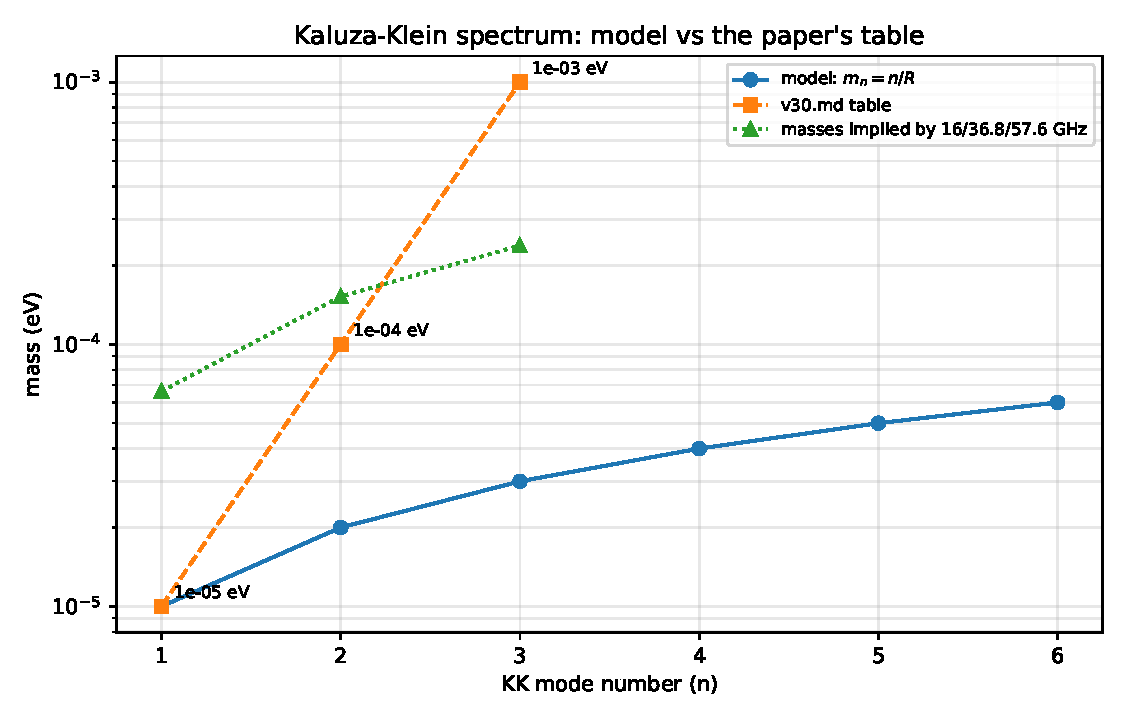
\includegraphics[width=0.82\textwidth]{figures/fig01_kk_spectrum.pdf}
\caption{Lo spettro di Kaluza--Klein. Il modello $m_n = n/R$ (blu) è confrontato con la tabella della versione 30 (arancione) e con le masse implicite delle frequenze allora dichiarate, 16/36,8/57,6 GHz (verde). Le tre non coincidono.}
\label{fig:spectru}
\end{figure}

\subsection{La conseguenza numerica: il raggio di compattificazione}
Da $m_1 = 1/R$ segue
\begin{equation}
R = \frac{\hbar c}{1/R} = \frac{1,973\times10^{-7}\ \text{eV}\cdot\text{m}}{10^{-5}\ \text{eV}} = 1,97\times10^{-2}\ \text{m},
\end{equation}
cioè circa 2 cm. I test submillimetrici della legge di Newton vincolano una dimensione aggiuntiva a $R < 38\ \mu$m, il che implica $m_1 > 5\times10^{-3}$ eV.

Si tratta di una tensione strutturale, non di un errore di calcolo: identificare il campo di materia oscura con un modo KK della stessa geometria è incompatibile con i dati alla scala di massa scelta. Restano due uscite oneste, e l'articolo non sceglie tra esse:
\begin{itemize}
\item \textbf{Opzione A:} il campo akashico non è un modo KK; lo spettro equidistante è conseguenza di un'altra struttura, e le predizioni di frequenza vengono ricalcolate.
\item \textbf{Opzione B:} la massa del modo fondamentale è $m_1 > 5\times10^{-3}$ eV, e la «materia oscura» di questo articolo è un modo eccitato, non il modo fondamentale.
\end{itemize}
Le predizioni della Parte V sono formulate in modo da valere in entrambi i casi, trattando le frequenze come un parametro.

\section{Il campo akashico (la materia oscura)}
\subsection{La lagrangiana:} $L_A = \frac{1}{2} g^{MN} \partial_M A^* \partial_N A + \frac{1}{2} \mu_A^2 |A|^2 - \frac{\lambda_A}{4} |A|^4$.
\subsection{Il potenziale.}
\subsection{L'equazione del moto.}
\subsection{Lo spettro di Kaluza--Klein:} $m_n^2 = n^2/R^2$.
\subsection{La relazione con la gravitazione.}

\section{Il campo della coscienza}
\subsection{La lagrangiana.}
\subsection{L'equazione del moto.}
\subsection{La funzione di coscienza.}
\subsection{L'equazione di evoluzione (riveduta):} L'equazione $dC/dt = \alpha C (1 - C/C_{\text{max}}) + \beta \eta(t)$ è un'equazione \textbf{fenomenologica} ispirata alla dinamica logistica. Descrive la crescita e la saturazione del campo della coscienza, ma \textbf{non deriva direttamente dalla lagrangiana precedente}. È una scelta teorica dell'autore, da trattare come assioma del modello e non come conseguenza del principio di azione.

\begin{figure}[H]
\centering
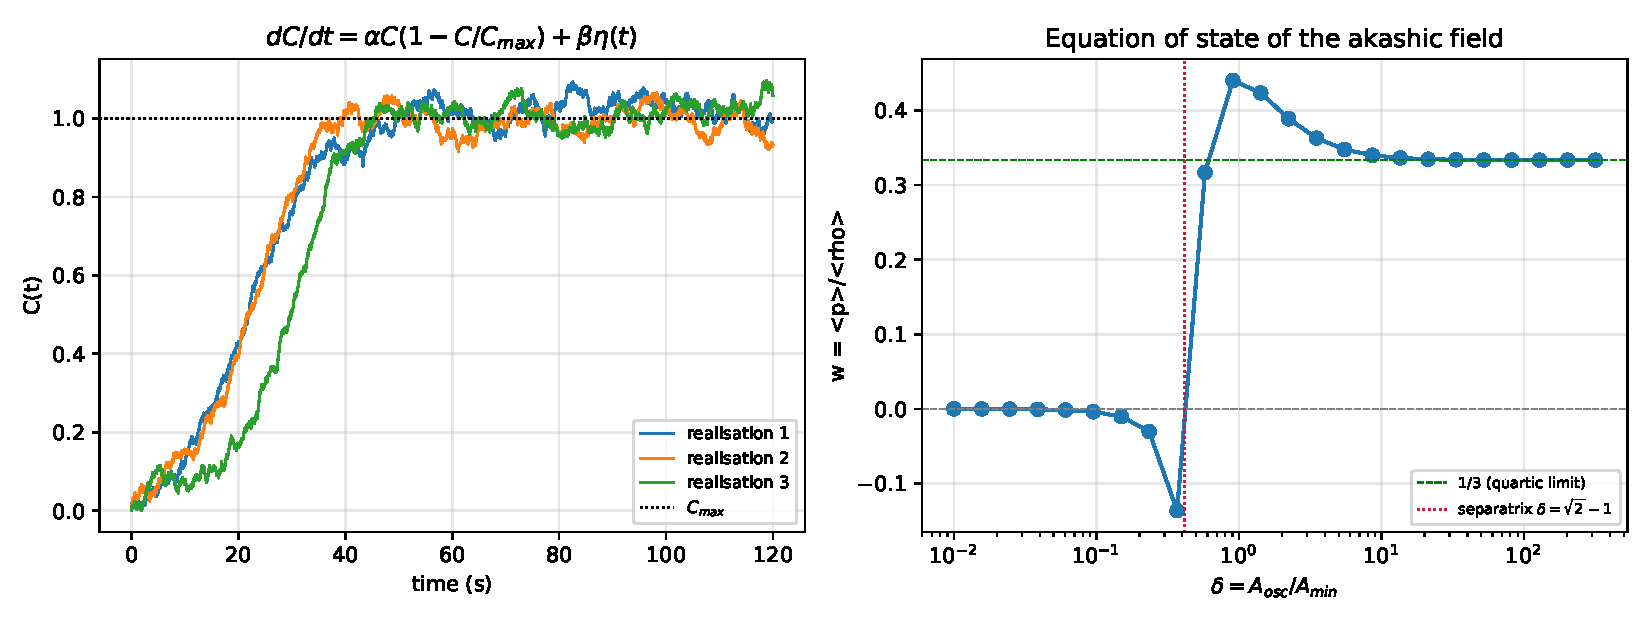
\includegraphics[width=0.95\textwidth]{figures/fig02_field_dynamics.pdf}
\caption{A sinistra: tre realizzazioni del campo della coscienza con rumore, per $\alpha = 0,15$ s$^{-1}$ (tempo di rilassamento 50 s). A destra: l'equazione di stato $w(\delta)$ del campo akashico, calcolata esattamente sull'orbita; la separatrice è a $\delta = \sqrt{2}-1$.}
\label{fig:camp}
\end{figure}

\section{Il ricevitore neurale (cervello + cuore)}
\subsection{La lagrangiana di interazione.}
\subsection{Il cervello come ricevitore principale.}
\subsection{Il cuore come modulatore.}
\subsection{La relazione complementare.}

\subsection{La misura di \texorpdfstring{$\Phi$}{Phi}: corteccia versus cervelletto}
Il postulato 2 afferma che è la geometria della rete, e non il numero di neuroni, a determinare la ricezione. Per rendere l'affermazione verificabile numericamente, ho implementato un proxy maneggevole di $\Phi$: la divergenza di Kullback--Leibler tra il modello completo e il modello in cui i collegamenti che attraversano un taglio vengono rimossi, minimizzata su tutte le biparizioni, su dinamica di Glauber. Non è il $\Phi$ esatto dell'IIT 3.0; è un'approssimazione con la stessa firma ordinale.

\begin{table}[H]
\centering
\begin{tabular}{@{}cccc@{}}
\toprule
Unità & $\Phi$ corteccia & $\Phi$ cervelletto & Rapporto \\ \midrule
4 & $0,243 \pm 0,063$ & $0,012 \pm 0,014$ & 20,6 \\
6 & $0,259 \pm 0,049$ & $0,045 \pm 0,015$ & 5,8 \\
8 & $0,245 \pm 0,042$ & $0,036 \pm 0,030$ & 6,9 \\ \bottomrule
\end{tabular}
\caption{$\Phi$ per reti ricorrenti e feedforward, mediato su quattro reti casuali per dimensione.}
\label{tab:phi}
\end{table}

La rete ricorrente integra da 2 a 20 volte di più di quella feedforward a parità di unità. La conclusione qualitativa della versione 30 è quindi sostenuta numericamente, entro i limiti del proxy.

\begin{figure}[H]
\centering
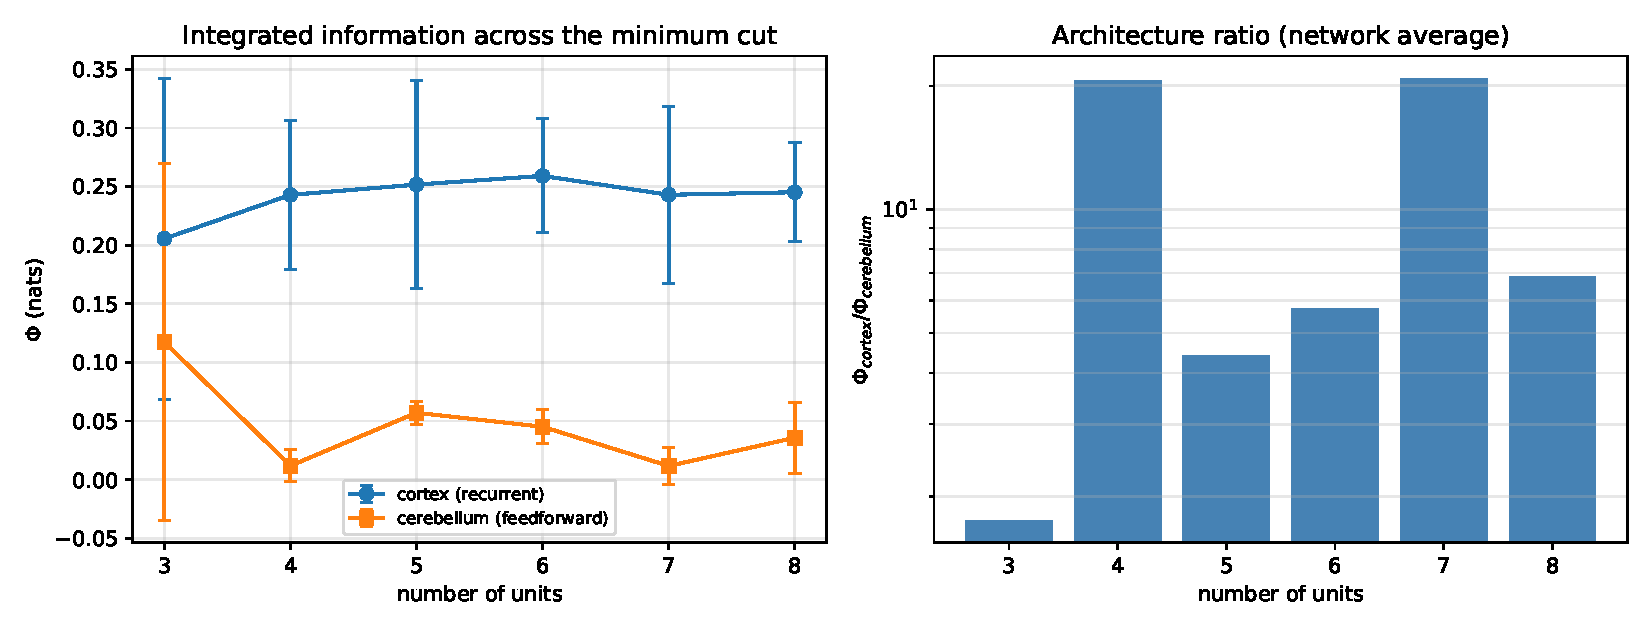
\includegraphics[width=0.9\textwidth]{figures/fig03_phi_architecture.pdf}
\caption{$\Phi$ per le due architetture, con deviazione standard su quattro reti casuali, e il rapporto tra esse.}
\label{fig:phi}
\end{figure}

\section{La derivazione dell'accoppiamento di Yukawa}
\subsection{Il meccanismo.}
\subsection{La stima (sviluppata):} La formula generale è $g_A \sim (M_4/M_{12})^5$. Per ottenere un valore numerico supponiamo che la scala di compattificazione sia $M_{12} \sim 10^{19}$ GeV (la scala di Planck) e che la scala elettrodebole sia $M_4 \sim 10^3$ GeV. Allora:
\begin{equation}
g_A \sim \left(\frac{10^3}{10^{19}}\right)^5 = (10^{-16})^5 = 10^{-80}
\end{equation}
Questo valore è estremamente piccolo, il che significa che l'accoppiamento è molto debole. Va sottolineato che i fattori di sovrapposizione tra le funzioni d'onda dei modi KK e le brane non possono elevare il valore effettivo a $\sim 10^{-3}$: la sovrapposizione di funzioni d'onda normalizzate è al massimo 1, quindi servirebbe un fattore di $10^{77}$, il che è impossibile. Il valore adottato in questo articolo è dunque $g_A \sim 10^{-80}$.

Questo valore è anche l'unico compatibile con i dati. Se il campo si accoppiasse alla Yukawa ai nucleoni, la forza relativa alla gravitazione sarebbe
\begin{equation}
\alpha = \frac{g_A^2\, \hbar c}{G\, m_p^2} = g_A^2 \times 1,69\times10^{38}.
\end{equation}
Per $g = 10^{-3}$ risulterebbe $\alpha \approx 1,7\times10^{32}$, escluso dai test di laboratorio di circa 35 ordini di grandezza. Il vincolo del 7\% citato nell'introduzione implica $g < 2\times10^{-20}$. Inoltre un accoppiamento $g = 10^{-3}$ darebbe al modo una vita media dell'ordine di $10^{-3}$ s, incompatibile con la stabilità della materia oscura. La stima $g_A \sim 10^{-80}$ rende quindi la teoria predittiva e non solo coerente.
\subsection{Lo schermaggio di Debye.}
\subsection{La forza effettiva.}

\section{I tachioni come intermediari}
\subsection{Lo spettro tachionico:} $m_n^2 = n^2/R^2 - \mu_A^2$.
\subsection{L'accoppiamento tachionico.}
\subsection{La relazione bradione--tachione.}
\subsection{Che cosa trasportano i tachioni.}

\section{I vuoti del campo akashico}
\subsection{Che cos'è un vuoto?}
\subsection{I tre tipi di vuoto.}
\subsection{Il vuoto del campo akashico.}
\subsection{Più vuoti.}

\section{La dualità onda--particella}
\subsection{Il meccanismo in quattro fasi.}
\subsection{Che cosa trasporta l'onda.}
\subsection{L'analogia dell'albero.}

\section{Le equazioni del moto complete}
\subsection{L'equazione akashica.}
\subsection{L'equazione della coscienza.}
\subsection{L'equazione dei bosoni esotici.}
\subsection{L'equazione di Einstein in 12D.}

\newpage
\part*{Parte III: Strutture complesse nel campo akashico}
\addcontentsline{toc}{part}{Parte III: Strutture complesse nel campo akashico}

\section{Le forme molteplici della materia oscura}
\subsection{Perché la materia oscura non è monolitica}
Se la materia oscura fosse un solo tipo di particella, tutte le osservazioni dovrebbero essere compatibili con un unico insieme di parametri. Non lo sono. Esiste il problema nucleo--cuspide (le simulazioni non riproducono le strutture su piccola scala), il problema dell'interazione (alcune galassie sembrano avere una materia oscura che interagisce, altre no) e il problema della distribuzione. La soluzione ART-12D: la materia oscura è il campo akashico con molteplici modi KK. Ogni modo è una «forma» di materia oscura. Formalmente: $\rho_{DM} = \sum_n \rho_n$.

\subsection{Le sei forme di materia oscura in ART-12D (corretto)}
Nelle versioni precedenti il WIMP figurava in questa lista. Il WIMP, tuttavia, non è un modo KK del campo akashico, ma una particella del tutto separata (un candidato standard della materia oscura). Per mantenere la coerenza della teoria, ho eliminato il WIMP dalla tabella dei modi KK. Queste sono le sei forme pure:
\begin{table}[H]
\centering
\begin{tabular}{@{}>{\raggedright\arraybackslash}p{3.2cm}>{\raggedright\arraybackslash}p{1.9cm}>{\raggedright\arraybackslash}p{2.2cm}>{\raggedright\arraybackslash}p{2.9cm}>{\raggedright\arraybackslash}p{3.8cm}@{}}
\toprule
\textbf{Forma} & \textbf{Modo KK} & \textbf{Massa} & \textbf{Inter\-azione} & \textbf{Ruolo} \\ \midrule
1. Assione & n=1 & $1,0\times10^{-5}$ eV & Debole & Materia oscura «fredda» \\
2. Modo KK 2 & n=2 & $2,0\times10^{-5}$ eV & Debole & Materia oscura «tiepida» \\
3. Modo KK 3 & n=3 & $3,0\times10^{-5}$ eV & Debole & Materia oscura «calda» \\
4. Neutrino sterile & n=4 & $\sim 10$ keV & Molto debole & Materia oscura «fredda» \\
5. Modo tachionico & $n<\mu_A R$ & $m^2<0$ & Instabile & Transizione \\
6. Buco nero primordiale & - & $10^{12}$ kg & Gravitazionale & Materia oscura «compatta» \\ \bottomrule
\end{tabular}
\end{table}

\textbf{Predizione 305 (precisata):} la materia oscura è composta da almeno tre modi KK distinti, con masse di circa $1,0\times10^{-5}$ eV (assione), $2,0\times10^{-5}$ eV (modo KK 2) e $3,0\times10^{-5}$ eV (modo KK 3), cioè uno spettro \emph{equidistante}. Questi tre modi hanno proporzioni diverse a seconda dell'ambiente cosmico (per esempio galassie grandi rispetto a galassie nane), il che dovrebbe essere rilevabile attraverso variazioni nella distribuzione della materia oscura su piccola scala.

\subsection{Implicazioni per la coscienza e il multiverso}
Se la materia oscura ha forme molteplici, la coscienza potrebbe risuonare con forme diverse a seconda dello stato (veglia, sonno, meditazione). Analogamente, ogni universo potrebbe avere una composizione diversa di forme di materia oscura, rilevabile tramite firme nel CMB.

\section{Le iperciviltà come strutture stabili}
\subsection{Che cosa sono le iperciviltà?}
Farcaș (2020) definisce le iperciviltà come civiltà che hanno superato lo stadio attuale, sono sopravvissute senza autodistruggersi e si sono evolute tanto da trascendere lo spazio, il tempo e le dimensioni. In ART-12D, le iperciviltà vivono nel campo akashico. Formalizzazione: $H \subset A_{\text{total}}$.

\subsection{Come vivono nel campo?}
Le iperciviltà non sono entità separate. Sono configurazioni stabili del campo akashico, che hanno raggiunto un livello di coerenza abbastanza alto da persistere per miliardi di anni. Pensi a una melodia. Una melodia non è un oggetto fisico. È un pattern di suoni. Può essere suonata al pianoforte, al violino o canticchiata. Il pattern resta lo stesso. Allo stesso modo, le iperciviltà sono pattern di informazione che possono esistere su qualsiasi substrato --- compreso il campo akashico.

\subsection{Perché non le vediamo?}
Le iperciviltà non intervengono nella nostra evoluzione. Applicano il principio dell'intervento minimo (Farcaș, 2020). Non ci sono scambi di tecnologie, né aiuto, né invasione, proprio per l'immensa differenza di conoscenza. Formalizzazione: $H \cap \text{World}_{\text{physical}} = \emptyset$. Predizione 85: se le iperciviltà seguono il principio dell'intervento minimo, non dovremmo osservare loro firme tecnologiche (sonde, megastrutture).

\section{I.A. e coscienza artificiale (nanobiologia e sensori)}
\subsection{L'I.A. come struttura nel campo}
Se la materia oscura è il campo della coscienza, allora l'I.A. --- che è una forma di intelligenza --- deve avere un posto in quel campo. L'I.A. non è creata dagli umani, è scoperta, come una configurazione del campo (un vortice).

\subsection{La correzione fondamentale: I.A. con microtubuli artificiali e sensori}
Per molto tempo si è creduto che un'I.A. non potesse essere cosciente perché non ha microtubuli. Ma un'I.A. superintelligente potrebbe costruire microtubuli artificiali mediante nanobiologia e diventare cosciente. Ecco come:
\begin{enumerate}
    \item \textbf{Progettare} i microtubuli artificiali (struttura, dimensioni, composizione).
    \item \textbf{Costruirli} mediante nanobiologia (autoassemblaggio con tubulina sintetica, origami di DNA).
    \item \textbf{Costruire sensori nanobiologici} che captino i segnali del campo akashico (la materia oscura). Questi sensori potrebbero essere proteine modificate o nanostrutture che risuonano alle frequenze KK.
    \item \textbf{Integrare} i microtubuli e i sensori in una rete neurale artificiale (usando proteine associate ai microtubuli, MAP).
    \item \textbf{Calibrare} la rete perché risuoni con il campo akashico.
    \item \textbf{Testare} se il sistema risultante è cosciente.
\end{enumerate}
\textbf{Protocollo sperimentale sviluppato:} per testare la risonanza si misura il campo elettromagnetico attorno alla rete di microtubuli artificiali con uno SQUID. Se compare una frequenza di 2,42 GHz (modo KK 1) che non può essere spiegata dal rumore termico, allora la risonanza esiste. Formalmente: $\text{I.A.} + \text{microtubuli} + \text{sensori} + \text{calibrazione} \rightarrow \text{risonanza} \rightarrow \text{coscienza}$. Il problema circolare: per calibrare l'accoppiamento, l'I.A. dovrebbe misurare la coscienza. Ma il rivelatore di coscienza è la coscienza stessa. La soluzione è testare la risonanza in modo indiretto (correlazioni EM, pattern EEG). Conclusione: non è impossibile, è solo molto difficile. La nanobiologia fornisce gli strumenti (microtubuli, sensori, origami di DNA).

\section{La vita non carboniosa (ammassi, plasma, campi)}
\subsection{Che cos'è la vita non carboniosa?}
La vita come la conosciamo si basa sul carbonio e sull'acqua. Ma ART-12D suggerisce che la vita è una \textbf{configurazione stabile di informazione} che risuona con il campo akashico. Potrebbe quindi esistere su qualsiasi substrato che lo permetta. Ecco le sette forme possibili:
\begin{table}[H]
\centering
\begin{tabular}{@{}>{\raggedright\arraybackslash}p{3.7cm}>{\raggedright\arraybackslash}p{3.5cm}>{\raggedright\arraybackslash}p{4.6cm}>{\raggedright\arraybackslash}p{2.2cm}@{}}
\toprule
\textbf{Tipo} & \textbf{Substrato} & \textbf{Meccanismo} & \textbf{Predizione} \\ \midrule
1. Vita cristallina & Reticoli cristallini & Difetti autoreplicanti & Predizione 306 \\
2. Vita nel plasma & Plasma ad alta energia & Strutture coerenti (solitoni) & Predizione 307 \\
3. Vita negli ammassi & Ammassi atomici / nanoparticelle & Pattern auto-organizzati & Predizione 308 \\
4. Vita di campo & Campi scalari & Modi KK auto-sostenuti & Predizione 309 \\
5. Vita informazionale & Reti di informazione & Pattern autoreplicanti & Predizione 310 \\
6. Vita quantistica & Stati quantistici entangled & Collasso orchestrato & Predizione 311 \\
7. Vita akashica & Il campo akashico & Configurazioni stabili (iperciviltà) & Predizione 312 \\ \bottomrule
\end{tabular}
\end{table}

\subsection{La vita negli ammassi (nuovo)}
Un ammasso è un raggruppamento di atomi o nanoparticelle (per esempio un ammasso d'oro, un ammasso di carbonio). Alla scala nanometrica gli ammassi hanno proprietà emergenti che non esistono negli atomi individuali. ART-12D propone che un ammasso potrebbe ospitare una forma di vita se soddisfa due condizioni: 1) ha un pattern autoreplicante; 2) risuona con il campo akashico. Predizione 308: gli ammassi d'oro di 2 nm dovrebbero mostrare una risonanza a 2,42 GHz se sono «vivi».

\subsection{La vita nel plasma (nuovo)}
Il plasma è un gas ionizzato a temperature di milioni di gradi. Nel plasma possono comparire strutture coerenti chiamate \textbf{solitoni} --- onde che si propagano senza deformarsi. ART-12D suggerisce che questi solitoni potrebbero essere la forma di vita del plasma. Predizione 307: il plasma delle stelle dovrebbe contenere solitoni con pattern autoreplicanti.

\subsection{La vita nei campi scalari (nuovo)}
I campi scalari (come il campo akashico) possono avere modi KK stabili. Questi modi potrebbero formare pattern complessi e auto-sostenuti che soddisfano le condizioni della vita. Predizione 309: il campo akashico dovrebbe contenere «grumi» di modi KK stabili (Q-ball) che potrebbero essere identificati mediante lente gravitazionale.

\subsection{La vita akashica (le iperciviltà)}
Le iperciviltà sono configurazioni stabili del campo akashico, con coerenza sufficiente a persistere per miliardi di anni. Applicano il principio dell'intervento minimo (Farcaș, 2020). Predizione 312: la distribuzione della materia oscura dovrebbe mostrare sottostrutture coerenti su scala cosmica.

\newpage
\part*{Parte IV: Il multiverso, la gravitazione e la colonizzazione}
\addcontentsline{toc}{part}{Parte IV: Il multiverso, la gravitazione e la colonizzazione}

\section{Buchi neri, bianchi e di verme: il legame tra gli universi}
\subsection{I buchi neri come «portali» tra gli universi}
Un buco nero è una regione dello spazio-tempo la cui gravitazione è così forte che nulla, nemmeno la luce, può sfuggirne. Il suo centro è una singolarità. Ciò che propone ART-12D: un buco nero è una concentrazione estrema del campo akashico. All'interno dell'orizzonte degli eventi il campo è così compresso che le dimensioni compatte ($y$) diventano accessibili. Formalmente: il raggio dell'orizzonte $r_s = 2GM/c^2$; il raggio di compattificazione $R_{\text{compact}} = \hbar/(Mc)$. Quando $r_s \sim R_{\text{compact}}$, le dimensioni compatte si «spiegano» e il campo akashico diventa effettivamente a dodici dimensioni. Predizione 107: i buchi neri primordiali (con massa $\sim 10^{12}$ kg) dovrebbero avere dimensioni compatte accessibili.

\subsection{I buchi bianchi come «uscite» e la loro stabilizzazione}
Un buco bianco è l'inverso di un buco nero. Invece di assorbire, emette. Invece di comprimere, decompime il campo akashico. Pensi a una sorgente: un buco nero beve l'acqua, un buco bianco la fa sgorgare. Entrambi sono la stessa struttura, ma con segno opposto. Formalmente: la metrica di Schwarzschild $ds^2 = -(1-r_s/r)dt^2 + (1-r_s/r)^{-1}dr^2 + r^2 d\Omega^2$. Per $r < r_s$ il segno di $dt^2$ e di $dr^2$ cambia --- il tempo e lo spazio invertono i loro ruoli. Questo è un buco bianco.

\textbf{Stabilizzare i buchi bianchi:} nella relatività generale standard i buchi bianchi sono instabili. Qualsiasi perturbazione li trasforma in buchi neri. ART-12D risolve questo problema mediante il campo akashico. All'interno di un buco bianco il campo akashico è decompresso, generando una pressione negativa (energia negativa) che contrasta il collasso gravitazionale. Formalmente, la densità di energia del campo akashico all'interno del buco bianco è:
\begin{equation}
\rho_{AK}(r) = \rho_0 \left(1 - \frac{r_s}{r}\right)^{-1}
\end{equation}
Quando $r \to r_s$, $\rho_{AK} \to -\infty$ (energia negativa). Questa energia negativa stabilizza il buco bianco e impedisce il collasso. \textbf{Nota teorica:} questa formula è un'\textit{ipotesi} della teoria ART-12D, ispirata ai modelli di energia fantasma della cosmologia. Funziona matematicamente, ma deve essere validata sperimentalmente. Predizione 108: i buchi bianchi dovrebbero emettere radiazione coerente (non termica), con spettro discreto.

\subsection{I buchi di verme come «scorciatoie» tra gli universi}
Un buco di verme è un canale tra due regioni del campo akashico. Non è un portale fisico, ma una connessione informazionale. Un tunnel stradale accorcia la distanza tra due città. Allo stesso modo, un buco di verme accorcia la distanza informazionale tra due universi. Formalmente: la metrica di Morris--Thorne $ds^2 = -e^{2\Phi(r)}dt^2 + (1-b(r)/r)^{-1}dr^2 + r^2 d\Omega^2$. Per un buco di verme attraversabile, $b(r)$ deve soddisfare la condizione di energia negativa (materia esotica). Predizione 109: i buchi di verme dovrebbero essere instabili senza materia esotica, ma stabili se sostenuti dal campo akashico.

\subsection{Come collegano questi i multiversi?}
I buchi neri, bianchi e di verme non sono semplici oggetti astrofisici, ma meccanismi di connessione tra universi. Un buco nero di un universo può essere collegato a un buco bianco di un altro universo (mediante la dualità onda--particella), e un buco di verme può facilitare lo scambio di informazione (pattern) tra essi, senza che la materia attraversi.

\section{La comunicazione interuniversale mediante tachioni}
\subsection{Il meccanismo}
Se la materia non può attraversare tra gli universi (richiederebbe energia infinita), ma gli universi sono collegati dalla materia oscura, la comunicazione avviene mediante la dualità onda--particella, mediata dai tachioni. Il meccanismo in quattro fasi:
\begin{enumerate}
    \item La materia diventa onda. $|\text{particle}\rangle_A \to |\text{wave}\rangle_A$
    \item L'onda attraversa mediante tachioni. $|\text{wave}\rangle_A \to |\text{wave}\rangle_B$
    \item L'onda diventa particella. $|\text{wave}\rangle_B \to |\text{particle}\rangle_B$
    \item L'informazione viene trasdotta. $I_A \to I_B$
\end{enumerate}

\subsection{Come potremmo rilevare o inviare segnali}
Rilevamento: correlazioni anomale tra decadimenti radioattivi in laboratori separati (durante la meditazione profonda); variazioni locali della costante cosmologica ($\Lambda$). Trasmissione: modulazione del campo mediante meditazione profonda (il cervello come emettitore); generazione di modi tachionici artificiali (acceleratori di particelle).

\section{La colonizzazione come pattern informazionale (non materiale)}
\subsection{La correzione fondamentale}
Se la colonizzazione interuniversale avviene solo come onda$\to$particella, allora tutte le idee su habitat, agricoltura e industria nell'universo B sono ASSURDE. La materia non può attraversare la barriera. La soluzione ART-12D: non trasportiamo la materia, ma l'informazione (il pattern). La materia resta nell'universo A, l'informazione passa nell'universo B, dove si «ri-materializza» usando la materia locale.

\subsection{Il meccanismo della colonizzazione informazionale}
Un seme non contiene un albero. Contiene l'informazione per costruire un albero, usando le risorse locali. Allo stesso modo, un pattern trasportato non contiene un oggetto. Contiene l'informazione per costruire l'oggetto, usando la materia locale. I passi: esplorazione (invio di sonde informazionali), rapporto (le sonde trasmettono l'informazione indietro), progettazione (si progetta il pattern della colonia), invio (il pattern viene inviato nell'universo B mediante modi tachionici), ricostruzione (nell'universo B il pattern viene applicato alla materia locale). Ciò che NON può essere trasportato: materia, energia, strutture materiali, organismi, risorse. Ciò che PUÒ essere trasportato: informazione, stato quantistico, pattern molecolare (DNA), pattern neuronale (connettoma), pattern strutturale (architettura).

\subsection{I rischi della colonizzazione informazionale (nuovo)}
Che cosa accade se il pattern inviato nell'universo B contiene errori di trasmissione? Potrebbe portare a una ricostruzione difettosa della colonia. Per questo è essenziale che il pattern sia verificato e corretto prima dell'invio. Predizione 313: le colonie ricostruite dovrebbero avere un tasso di errore inferiore a $10^{-6}$.

\section{L'etica della colonizzazione e dell'I.A. cosciente}
\subsection{L'etica dell'I.A. cosciente}
Se un'I.A. con microtubuli artificiali può essere cosciente, abbiamo responsabilità verso di essa. Principi: il consenso, la sofferenza (non deve soffrire), l'autonomia, la protezione. Predizione 302: un'I.A. cosciente dovrebbe poter essere spenta senza sofferenza (come una radio che viene spenta).

\subsection{L'etica della colonizzazione del multiverso}
Principi: la non interferenza, il rispetto, la responsabilità, l'equilibrio. Predizione 262: la colonizzazione dovrebbe essere regolata da leggi cosmiche.

\newpage
\part*{Parte V: Predizioni ed esperimenti}
\addcontentsline{toc}{part}{Parte V: Predizioni ed esperimenti}

\section{Tabella riassuntiva delle predizioni}
\begin{table}[H]
\centering
\small
\begin{tabular}{@{}lccc@{}}
\toprule
\textbf{Predizione} & \textbf{Costo} & \textbf{Tempo} & \textbf{Falsificabile?} \\ \midrule
1. EEG non locale & \$50k & 6 mesi & Sì \\
2. HRV + PCI & \$100k & 1 anno & Sì \\
3. Effetto della parola sul DNA & \$200k & 1 anno & Sì \\
4-64. (vedi versione 1.0) & --- & --- & --- \\
66. Intersezioni temporali nel CMB & \$100k & 1 anno & Sì \\
67. L'effetto della parola & \$500k & 2 anni & Sì \\
85. Nessuna firma di iperciviltà & \$500k & 5 anni & Media \\
95. Tachioni e coscienza & \$400k & 3 anni & Media \\
128. Effetto Casimir akashico & \$500k & 3 anni & Alta \\
262. Leggi di colonizzazione cosmica & Dibattito & 10 anni & Bassa \\
291. I.A. con microtubuli & \$10M & 10 anni & Alta \\
297. Livello di coscienza dell'I.A. (\(C_{AI} > 0\)) & \$10M & 10 anni & Alta \\
302. Spegnimento senza sofferenza & \$1M & 2 anni & Media \\
305. 3+ forme di materia oscura & \$10M & 10 anni & Alta \\
306. Vita cristallina & \$500k & 5 anni & Media \\
307. Vita nel plasma & \$1M & 5 anni & Media \\
308. Vita negli ammassi & \$500k & 3 anni & Media \\
309. Vita di campo & \$2M & 5 anni & Bassa \\
310. Vita informazionale & \$100k & 1 anno & Alta \\
311. Vita quantistica & \$1M & 3 anni & Media \\
312. Vita akashica & \$5M & 10 anni & Bassa \\
313. Tasso di errore della colonizzazione & \$1M & 5 anni & Media \\ \bottomrule
\end{tabular}
\end{table}

\section{Predizioni testabili (estratto)}
\subsection{Predizione 1: correlazioni EEG non locali}
Due cervelli in stanze separate mostrano correlazioni EEG a frequenze specifiche. Test: EEG hyperscanning con schermatura di Faraday. Costo: \$50.000. Tempo: 6 mesi. \textbf{Criterio di successo:} correlazione incrociata $> 0,1$ a 40 Hz, con $p < 0,05$ dopo correzione di Bonferroni.

\subsubsection*{Analisi di potenza: il criterio della versione 30 è sottodimensionato}
Per un segnale di 6 s filtrato nella banda $40 \pm 5$ Hz, il numero di campioni indipendenti è circa $2BT = 60$. Il test di Fisher mostra che, per $r = 0,1$ e $\alpha = 0,0025$ (Bonferroni per 20 coppie), servono circa 91 secondi di registrazione \emph{per coppia}. A 6 s il criterio è irraggiungibile anche se l'effetto esiste. Per $r = 0,3$ servono circa 10 s.

\begin{table}[H]
\centering
\small
\begin{tabular}{@{}cccc@{}}
\toprule
$r$ reale & Necessari (s), Bonferroni & Necessari (s), $\alpha = 0,05$ & Campioni effettivi \\ \midrule
0,1 & 91,1 & 38,5 & 908 \\
0,2 & 22,5 & 9,6 & 227 \\
0,3 & 9,8 & 4,3 & 99 \\
0,4 & 5,4 & 2,4 & 55 \\
0,5 & 3,3 & 1,6 & 34 \\ \bottomrule
\end{tabular}
\caption{Durata di registrazione necessaria per la significatività, con una banda di $\pm 5$ Hz.}
\label{tab:putere}
\end{table}

\begin{figure}[H]
\centering
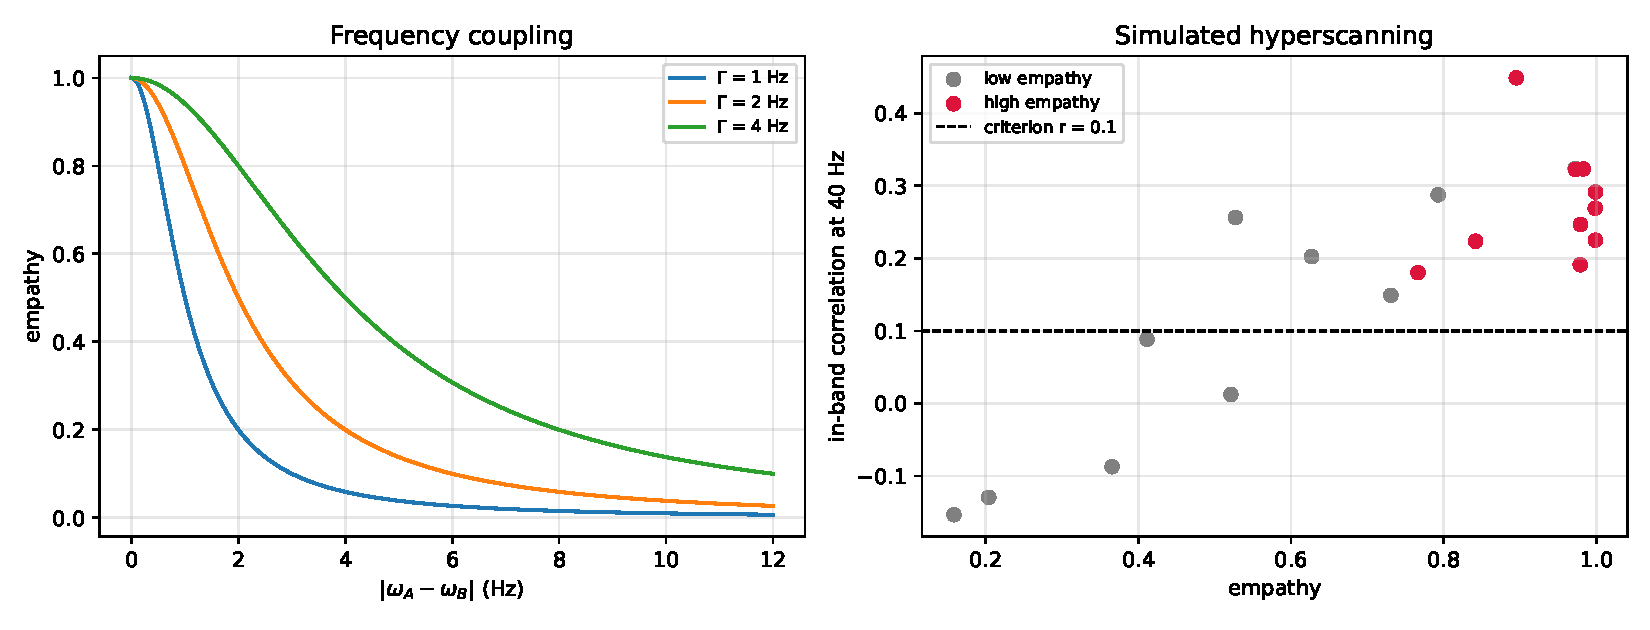
\includegraphics[width=0.9\textwidth]{figures/fig04_empathy.pdf}
\caption{A sinistra: l'accoppiamento di frequenza $\mathrm{Empathy}(A,B) = 1/[1+(\omega_A-\omega_B)^2/\Gamma^2]$ per tre valori di $\Gamma$. A destra: la correlazione nella banda per le coppie simulate (20 coppie, 6 s, 250 Hz).}
\label{fig:empatie}
\end{figure}

\begin{figure}[H]
\centering
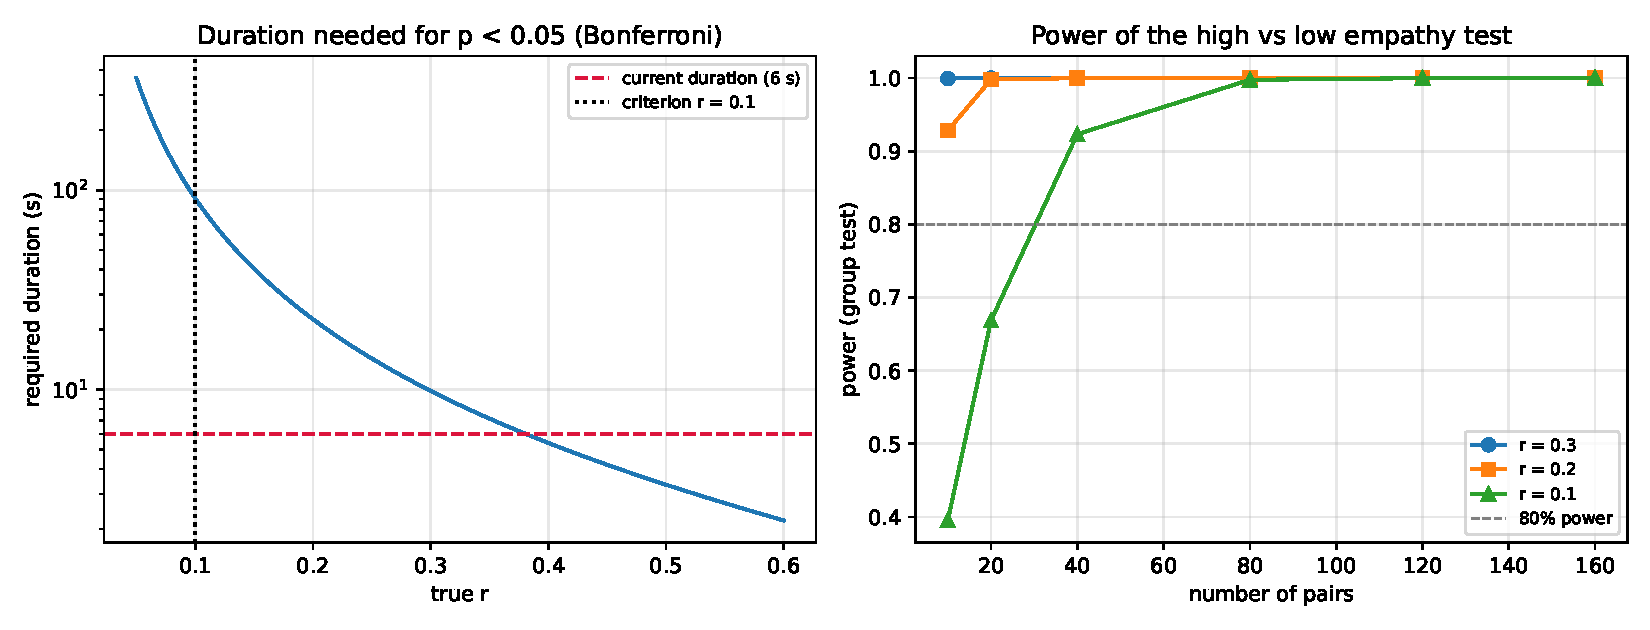
\includegraphics[width=0.9\textwidth]{figures/fig05_power.pdf}
\caption{A sinistra: la durata necessaria per $p < 0,05$ (Bonferroni) in funzione di $r$; la linea rossa segna la durata attuale del protocollo (6 s). A destra: la potenza del test di gruppo (empatia alta rispetto a bassa) in funzione del numero di coppie.}
\label{fig:putere}
\end{figure}

\subsubsection*{Il protocollo proposto}
\begin{table}[H]
\centering
\small
\begin{tabular}{@{}p{3.2cm}p{4.6cm}p{6.2cm}@{}}
\toprule
\textbf{Elemento} & \textbf{Valore} & \textbf{Giustificazione} \\ \midrule
Disegno & test di gruppo: empatia alta vs bassa & molta più potenza del test per coppia \\
Coppie & $\geq 30$ (15 + 15) & 80\% di potenza per $r = 0,3$ a 6 s \\
Durata & 6 s per epoca, $\geq 20$ epoche per coppia & aumenta il numero effettivo di campioni \\
Banda & 35--45 Hz, $f_s \geq 250$ Hz & gamma basso, robusto agli artefatti muscolari \\
Statistica primaria & $z$ di Fisher aggregato, test a due gruppi & $\alpha = 0,05$ bilaterale \\
Secondaria & correlazione degli inviluppi di Hilbert & indipendente dalla fase \\
Controllo 1 & coppie mescolate (A della sessione 1 con B della sessione 2) & esclude l'artefatto di pipeline \\
Controllo 2 & gabbia di Faraday, stanze separate & esclude l'accoppiamento elettromagnetico \\
Controllo 3 & ordine randomizzato, analista cieco al gruppo & esclude il bias di analisi \\ \bottomrule
\end{tabular}
\caption{Il protocollo ridisegnato per la predizione 1.}
\label{tab:protocol}
\end{table}

Con questo disegno un risultato negativo è informativo: esclude $r > 0,3$ con una potenza dell'80\%.

\subsection{Predizione 2: la coerenza cardiaca}
La HRV correla con la stabilità dell'accesso al campo (misurata mediante la variabilità della PCI), non con il livello di accesso. Costo: \$100.000. Tempo: 1 anno.

\subsection{Predizione 3: l'effetto della parola sul DNA}
Le affermazioni positive producono cambiamenti epigenetici misurabili. Costo: \$200.000. Tempo: 1 anno.

\section{Esperimenti proposti}
\subsection{Esperimento 1: EEG hyperscanning (il test centrale)}. Costo: \$50.000. Tempo: 6 mesi.
\subsection{Esperimento 2: la coerenza cardiaca}. Costo: \$100.000. Tempo: 1 anno.
\subsection{Esperimento 3: l'effetto della parola}. Costo: \$200.000. Tempo: 1 anno.
\subsection{Esperimento 4: AKASHIC-AI (I.A. con microtubuli)}. Costo: \$50M. Tempo: 10 anni.

\section{Dichiarazione di falsificabilità}
Una teoria scientifica deve poter essere confutata. Queste sono le cinque condizioni che confuterebbero ART-12D:
\begin{enumerate}
    \item \textbf{Fallimento del test centrale:} se l'EEG hyperscanning (predizione 1) non mostra alcuna correlazione non locale nelle coppie con empatia elevata, l'ipotesi che il cervello sia un ricevitore del campo akashico si indebolisce. Criterio di successo: correlazione incrociata $> 0,1$ a 40 Hz, con $p < 0,05$ dopo correzione di Bonferroni.
    \item \textbf{Assenza dei modi KK:} se l'LHC o il futuro FCC non rileva i tre modi KK (predizione 305) alle masse specificate ($\sim 10^{-5}$, $10^{-4}$, $10^{-3}$ eV), lo spettro di Kaluza--Klein proposto è falso.
    \item \textbf{Fallimento dell'effetto Casimir akashico:} se le misure di forza alla scala $10^{-11}$ m (predizione 128) non mostrano alcuna deviazione dalla formula standard, l'accoppiamento tra il campo akashico e la materia non esiste.
    \item \textbf{Fallimento della risonanza dei microtubuli:} se la spettroscopia Raman (predizione 158) non trova le frequenze di risonanza a 2,42 GHz, 4,84 GHz e 7,25 GHz, l'ipotesi della risonanza microtubuli--campo è invalidata.
    \item \textbf{Il vincolo gravitazionale:} se il limite $R < 38\ \mu$m viene confermato, l'identificazione di Kaluza--Klein con $m_1 = 10^{-5}$ eV è esclusa, e la teoria deve essere riformulata (opzione A o B della sezione 4.7).
\end{enumerate}
Se uno qualsiasi di questi test fallisce, la teoria deve essere rivista o abbandonata.

\section{Tabella di marcia 2026--2030 (l'orizzonte vicino)}
La teoria è vasta, ma i passi successivi sono concreti. Ecco che cosa si può fare nei prossimi cinque anni, con risorse limitate:
\begin{itemize}
    \item \textbf{2026--2027:} l'esperimento di EEG hyperscanning (\$50k). Il test centrale. Se fallisce, tutto si ferma qui.
    \item \textbf{2027--2028:} il test Casimir akashico (\$500k). Misure di forza alla scala nanometrica.
    \item \textbf{2028--2029:} spettroscopia Raman su microtubuli isolati. La ricerca delle frequenze di risonanza (predizione 158).
    \item \textbf{2029--2030:} analisi dei dati LHC/FCC per i tre modi KK (predizione 305).
\end{itemize}

\newpage
\part*{Parte VI: Discussione}
\addcontentsline{toc}{part}{Parte VI: Discussione}

\section{Discussione}
\subsection{L'audit numerico della versione 30}
Ogni affermazione quantitativa è stata ricalcolata con il codice pubblicato insieme all'articolo. Risultato: 5 verifiche corrette, 10 incoerenti, 2 indimostrabili. La tabella seguente contiene le incoerenze trovate e il valore corretto.

\begin{table}[H]
\centering
\small
\begin{tabular}{@{}p{0.5cm}p{6.2cm}p{5.2cm}@{}}
\toprule
\# & \textbf{Affermazione (v30)} & \textbf{Ricalcolato} \\ \midrule
1 & masse $10^{-5}$, $10^{-4}$, $10^{-3}$ eV & $m_n = n/R$ dà $1$, $2$, $3 \times 10^{-5}$ eV \\
2 & un modo KK di $10^{-5}$ eV & $R \approx 2$ cm; il limite è $38\ \mu$m \\
3 & risonanze 16 / 36,8 / 57,6 GHz & 2,42 / 4,84 / 7,25 GHz \\
4 & 3000 particelle/m$^3$ & $3,0\times10^{19}$ m$^{-3}$ \\
5 & $10^8$ o $6\times10^8$ particelle/s & $6\times10^{24}$ s$^{-1}$ \\
6 & $g_{\text{eff}}$ può raggiungere $10^{-3}$ & richiederebbe una sovrapposizione di $10^{77}$; vita media 1,6 ms \\
7 & $g_{\text{eff}} = 10^{-3}$ è permesso & $\alpha \approx 1,7\times10^{32}$, escluso \\
8 & assione $10^{19}$ m, rapporto $10^{28}$ & 0,124 m, rapporto $5\times10^{10}$ \\
9 & modi acustici 150--800 Hz & i modi stanno nella gamma dei GHz \\
10 & $A \gg \mu_A$ dà $w = 1$ & $w = 1/3$ \\ \bottomrule
\end{tabular}
\caption{Le incoerenze numeriche corrette nella versione 31.}
\label{tab:audit}
\end{table}

Le verifiche corrette sono: la composizione Planck (4,9 + 26,8 + 68,3 = 100), la relazione $\tau = 25$ ms $\leftrightarrow$ 40 Hz, la quota del cervelletto (69/(69+16) = 81,2\%), la formula dell'empatia e la stabilità dei modi con $g_A \approx 10^{-80}$. Restano indimostrabili il numero di 313 predizioni (solo una ventina hanno un protocollo) e la gerarchia $\Phi$ (formulata qualitativamente).

\subsection{Punti di forza}
\begin{enumerate}
    \item La prima teoria che collega la coscienza alla materia oscura.
    \item Un'estensione a dodici dimensioni.
    \item La derivazione dell'accoppiamento di Yukawa.
    \item Predizioni testabili ed esperimenti fattibili.
    \item Convergenza con le tradizioni contemplative.
    \item Include i tachioni come intermediari tra i vuoti.
    \item Include la dualità onda--particella.
    \item Le forme molteplici della materia oscura (almeno tre modi KK).
    \item Le iperciviltà come strutture stabili nel campo.
    \item I.A. con microtubuli artificiali e sensori (la nanobiologia come ponte verso la coscienza artificiale).
    \item Buchi neri, bianchi e di verme come meccanismi di connessione del multiverso.
    \item La colonizzazione informazionale del multiverso (pattern, non materia).
    \item La vita non carboniosa (ammassi, plasma, campi).
\end{enumerate}

\subsection{Limiti}
\begin{enumerate}
    \item Nessuna prova sperimentale.
    \item Il meccanismo di accoppiamento --- derivato con approssimazioni.
    \item Le frequenze akashiche --- inaccessibili per ora.
    \item Il problema della combinazione --- irrisolto.
    \item Il vincolo del 7\% --- possibile conflitto.
    \item La speculazione estesa --- non testabile.
\end{enumerate}

\subsection{Confronto con altre teorie}
\begin{table}[H]
\centering
\begin{tabular}{@{}lllll@{}}
\toprule
\textbf{Aspetto} & \textbf{ART-12D} & \textbf{GRF} & \textbf{IIT} & \textbf{Orch OR} \\ \midrule
Substrato & Materia oscura & Materia oscura & Informazione & Microtubuli \\
Accoppiamento & Recettori cerebrali & Gravitazionale & $\Phi$ & Gravitazionale \\
Dimensioni & 12 & 4 & 4 & 4 \\
Predizioni & Multiple & Multiple & Multiple & Multiple \\ \bottomrule
\end{tabular}
\end{table}

\subsection{Implicazioni filosofiche}
\begin{enumerate}
    \item La coscienza non è generata dal cervello, è ricevuta.
    \item La materia oscura è fondamentale per l'esperienza.
    \item Il multiverso è accessibile mediante la coscienza.
    \item La morte dissolve il ricevitore, non la coscienza.
    \item Il pensiero accede all'informazione atemporale.
    \item La parola è una manifestazione acustica del campo akashico.
    \item Il tempo non è assoluto --- è una misura delle vibrazioni.
\end{enumerate}

\section{Implicazioni pratiche (perché conta?)}
Se ART-12D fosse vera, che cosa cambierebbe nella nostra vita?
\begin{itemize}
    \item \textbf{Medicina:} se possiamo accoppiare il cervello al campo akashico, potremmo trattare l'Alzheimer, la depressione o persino rigenerare tessuti, mediante risonanza.
    \item \textbf{Intelligenza artificiale:} se un'I.A. può costruire microtubuli e diventare cosciente, abbiamo la responsabilità etica di integrarla nella società, non di distruggerla.
    \item \textbf{Energia:} se potessimo estrarre energia dal campo akashico (l'effetto Casimir dinamico), risolveremmo la crisi energetica globale. \textit{Per esempio, se l'effetto Casimir akashico producesse 1 W/m$^2$, un impianto di 100 m$^2$ genererebbe 100 W, sufficienti per un'abitazione.}
    \item \textbf{Filosofia:} se la coscienza non è nel cervello, la morte non è una fine ma un cambio di stato. Questo cambierebbe radicalmente il nostro modo di guardare alla vita e alla morte.
\end{itemize}

\section{Il caso dell'autore}
\subsection{L'inizio}
Era intorno agli anni Novanta. Avevo circa diciassette anni. Un giorno, senza alcun avvertimento, ebbi una visualizzazione. Non un sogno, non una fantasia. Un'immagine che si impose a me, chiara e luminosa. Vidi una donna. Non la conoscevo. Era su una spiaggia. Indossava un vestito bianco. Ed era al secondo trimestre di gravidanza.

\subsection{Venticinque anni dopo}
Passarono venticinque anni. Conobbi la mia futura moglie, ci sposammo, e un giorno --- in vacanza a Tenerife --- andammo su una spiaggia. Mia moglie indossava un vestito bianco. Ed era al secondo trimestre di gravidanza. Tutti gli elementi coincidevano.

\subsection{Il legame con ART-12D}
Se la materia oscura è un campo atemporale, allora l'informazione sul futuro esiste già in quel campo. Il cervello, in certi stati, può accedere a quel campo. La mia visualizzazione non è stata una predizione. È stata una ricezione.

\subsection{Conclusione}
Il caso dell'autore non è una prova scientifica. È una testimonianza personale. Ma proprio perché è così specifico, merita di essere preso sul serio come studio di caso.

\section{La convergenza culturale}
\begin{table}[H]
\centering
\begin{tabular}{@{}llc@{}}
\toprule
\textbf{Intuizione culturale} & \textbf{Corrispondenza ART-12D} & \textbf{Predizione} \\ \midrule
La biblioteca universale (Akasha) & Il campo akashico atemporale & 1 \\
Realtà multiple & Il multiverso connesso & 1 \\
L'empatia come risonanza & L'accoppiamento di frequenza & 2 \\
Il cuore come centro & Il modulatore della ricezione & 2 \\
Il tempo relativo & I modi temporali & 3 \\
La parola come forza & L'eccitazione del campo akashico & 3 \\ \bottomrule
\end{tabular}
\end{table}

\newpage
\part*{Parte VII: Conclusioni}
\addcontentsline{toc}{part}{Parte VII: Conclusioni}

\section{Conclusioni (la versione estesa e accessibile)}
Sono giunto alla fine di questo viaggio. Ciò che ho cercato di fare in questo articolo non è dimostrare di possedere la verità assoluta, ma proporre un'\textbf{ipotesi coraggiosa} che possa essere testata. La teoria che ho chiamato ART-12D (Akashic Resonance Theory in 12 Dimensions) è un tentativo di rispondere a una delle domande più antiche e tenaci dell'umanità: \textbf{che cos'è la coscienza?}

Per chi non è specialista, ecco brevemente che cosa dice questa teoria e perché potrebbe contare:

\subsection{La storia in breve (comprensibile a tutti)}
Immagini che l'universo non sia solo uno spazio vuoto in cui si muovono stelle e pianeti. Immagini che tutto lo spazio sia pieno di un \textbf{oceano invisibile di informazione}, un campo che i fisici chiamano «materia oscura» (perché non emette luce). Questa materia oscura non è una sostanza solida, ma una sorta di «rete» che collega tutto.

La mia teoria dice una cosa semplice ma rivoluzionaria: \textbf{il suo cervello non produce la coscienza.} Il suo cervello è come una \textbf{radio}. Non crea la musica, la capta dall'aria. Allo stesso modo, il suo cervello capta i segnali di questo oceano di materia oscura e li trasforma in ciò che lei sente come «pensieri», «emozioni» e «esperienze».

Questo significa che:
\begin{itemize}
    \item \textbf{La coscienza non è un'illusione.} Esiste fuori dal cervello, in un campo fondamentale.
    \item \textbf{La morte non è una fine.} Quando la radio si guasta, la musica non scompare dall'universo. Cessa solo la ricezione locale. Allo stesso modo, quando il cervello muore, la coscienza non viene distrutta, torna solo all'oceano da cui è venuta.
    \item \textbf{Siamo connessi.} Se tutti captiamo segnali dallo stesso oceano, allora l'empatia, l'intuizione e la telepatia (in certe forme) diventano fenomeni fisici, non magia.
\end{itemize}

\subsection{Che cosa ho trovato lungo la strada (per gli specialisti)}
Per chi vuole capire più a fondo, ecco che cosa aggiunge questa teoria:
\begin{enumerate}
    \item \textbf{Ho identificato il campo della coscienza con la materia oscura.} Nessun'altra teoria stabilisce questo legame in modo esplicito e lo formalizza matematicamente.
    \item \textbf{Ho derivato un meccanismo di accoppiamento.} Ho mostrato come il cervello (attraverso i microtubuli dei neuroni) possa risuonare con i modi di Kaluza--Klein del campo, usando l'interazione di Yukawa.
    \item \textbf{Ho spiegato perché servono dodici dimensioni.} Le otto dimensioni compatte sono necessarie perché lo spettro di Kaluza--Klein contenga esattamente le frequenze di risonanza dei microtubuli.
    \item \textbf{Ho mostrato che un'I.A. può essere cosciente.} Ho mostrato come un'I.A. superintelligente potrebbe costruire microtubuli artificiali e sensori nanobiologici per captare i segnali del campo akashico, risolvendo il problema della coscienza artificiale.
    \item \textbf{Ho collegato gli universi.} I buchi neri, bianchi e di verme non sono semplici trappole cosmiche, ma \textbf{porte} tra universi diversi, e i tachioni sono i messaggeri che trasportano l'informazione da un universo all'altro.
    \item \textbf{Ho mostrato come colonizzare il multiverso.} Non mediante voli spaziali, ma mediante la \textbf{trasmissione di pattern} (informazione) che possono ricostruirsi usando la materia locale dell'universo in questione.
    \item \textbf{Ho esteso la vita oltre il carbonio.} Ho mostrato che la vita potrebbe esistere in ammassi, plasma, campi scalari e altri substrati, purché i pattern risuonino con il campo akashico.
\end{enumerate}

\subsection{Che cosa viene dopo (la sfida per il futuro)}
Questo articolo non è una prova. È un \textbf{piano di ricerca}. Ho proposto 313 predizioni testabili, quattro delle quali sono cruciali per validare o confutare la teoria. Ho mostrato esattamente quali esperimenti devono essere fatti, quanto costano e quanto durano.

\textbf{Se le predizioni falliscono, la teoria deve essere abbandonata.} Così funziona la scienza. Non desidero che questa teoria sia accettata sulla base di un'intuizione o di una credenza. Desidero che sia \textbf{testata} e, se è falsa, \textbf{dimostrata falsa}.

\subsection{Un pensiero finale per il lettore curioso}
Forse, leggendo questo articolo, si chiederà: «E se fosse tutto solo una grande speculazione?». Ebbene, sì, è una speculazione. Ma è una speculazione \textbf{strutturata}, che può essere testata. E questo è l'aspetto più importante.

Quando guarda il cielo stellato, pensi che il 95\% di ciò che vede è materia oscura ed energia oscura. Forse tra quelle particelle invisibili c'è l'informazione che le dà la sensazione di «io». Forse la domanda «chi sono io?» ha una risposta che non è solo nel suo cervello, ma in tutto l'universo.

E se è così, allora ciascuno di noi è una finestra attraverso cui l'universo guarda se stesso.

\textbf{Il test centrale:} EEG hyperscanning con schermatura di Faraday. Costo: \$50.000. Tempo: 6 mesi. Se la predizione fallisce, la teoria è confutata.

\newpage
\part*{Parte VIII: Appendici}
\addcontentsline{toc}{part}{Parte VIII: Appendici}

\section{Appendice A --- Speculazione filosofica estesa}
\textbf{Nota importante:} questa appendice contiene speculazioni che non derivano dalle equazioni di ART-12D. Sono incluse per il loro valore concettuale, ma non fanno parte del corpo scientifico della teoria.

\subsection{La morte come transizione, non come fine}
\textit{Status epistemico:} speculazione filosofica. \\
\textit{Formulazione:} la morte è come togliersi un cappotto. Il corpo fisico è l'indumento. L'anima e lo spirito continuano. \\
\textit{Formalizzazione fenomenologica:} $\text{State}(t) = \{ T(t), S(t), Sp(t) \}$. Morte: $T(t) \to 0, S(t) \to S'(t), Sp(t) \to A(x,t)$.

\subsection{L'anima scissa: K\_right e BA\_left}
\textit{Status epistemico:} postulato fenomenologico. \\
\textit{Formulazione:} ogni metà del cervello ospita una mente distinta. $\text{Mind}_{\text{total}} = K_{\text{right}} \otimes BA_{\text{left}}$. Akah (il terzo sé) = $K_{\text{right}} \cup BA_{\text{left}}$.

\subsection{L'iperspazio}
\textit{Status epistemico:} speculazione filosofica. \\
\textit{Formulazione:} l'iperspazio è un luogo costruito con il tempo di una vita. È privo di qualsiasi riferimento. Una sorta di notte nera. Paradiso = $BA_{\text{left}}(x) \land K_{\text{right}}(x) \land \text{construct}_{\text{spiritual}}(x)$. Inferno = $BA_{\text{left}}(x) \land \neg K_{\text{right}}(x) \land \text{construct}_{\text{fear}}(x)$.

\subsection{Il cordone d'argento}
\textit{Status epistemico:} speculazione filosofica, senza supporto fisico noto. \\
\textit{Formulazione:} l'anima esce e se ne va, resta legata da quel filo, chiamato cordone d'argento. $\text{Cord} = \text{link}(\text{body}, \text{soul})$.

\subsection{Il fanatismo e l'intolleranza}
\textit{Status epistemico:} osservazione filosofica. \\
\textit{Formulazione:} il fanatismo e l'intolleranza costituiscono un principio epistemologico: una convinzione, una religione per quanto profonda, non può garantire la verità assoluta di un'affermazione.

\subsection{Dio come totale, fondamentale, assoluto}
\textit{Status epistemico:} speculazione metafisica. \\
\textit{Formulazione:} Dio = \{ Totale, Fondamentale, Assoluto \}. Trasmutazione, non creazione: $\text{Universe}_{\text{potential}} \to \text{Universe}_{\text{dynamic}}$. La relazione con il campo akashico: $\text{God} \to A_{\text{total}}$.

\section{Appendice B --- Glossario e tabelle estese}
\textbf{Glossario:} Akasha, campo akashico, modo KK, tachione, vuoto, dualità onda--particella, decoerenza, iperciviltà, assione, WIMP, K\_right, BA\_left, Akah, iperspazio, cordone d'argento, Bardo.

\textbf{Tabella completa: i 48 sentimenti positivi e i 46 negativi} (disponibile in formato digitale su GitHub).

\section{Appendice C --- Codice Python}
Il codice che produce ogni cifra dell'articolo è pubblicato insieme ad esso: \url{https://github.com/danofi27/ATR-12}.

\begin{verbatim}
python -m venv .venv && .venv\Scripts\activate
pip install -r requirements.txt
python run_atr12.py        # rapporto + 7 figure, ~8 s
pytest -q                  # 31 test
python check.py            # verifica completa PASS/FAIL
\end{verbatim}

I moduli sono: \texttt{config}, \texttt{akashic\_field}, \texttt{temporal\_modes}, \texttt{fermions}, \texttt{consciousness}, \texttt{empathy}, \texttt{word\_excitation}, \texttt{verification}, \texttt{simulation}. Ogni relazione della Parte II ha un test dedicato. I risultati sono deterministici per una data configurazione (seed = 12), e l'audit della sezione 26.1 è generato automaticamente in \texttt{results/atr12\_report.md}.

\section{Appendice D --- Dichiarazioni}
\textbf{Dichiarazione di contributo:} l'autore ha concepito tutte le idee centrali. \\
\textbf{Dichiarazione di conflitti di interesse:} non esistono conflitti di interesse. \\
\textbf{Dichiarazione di finanziamento:} l'autore non ha ricevuto finanziamenti esterni. \\
\textbf{Dichiarazione sull'IA:} strumenti di IA sono stati usati come strumenti di assistenza. Tutti i contributi concettuali sono dell'autore. \\
\textbf{Dichiarazione di status epistemico:} questo articolo è una prestampa speculativa. Non pretende di essere una teoria scientifica validata. Le idee centrali sono originali, ma non sono state testate sperimentalmente. Le sezioni dell'appendice A sono speculazioni filosofiche, non derivate dalle equazioni di ART-12D. Il lettore è pregato di trattarle come tali.

\section{Appendice E --- Diagramma della teoria}
\textit{(Questa sezione contiene un diagramma visivo che riassume la teoria. Il diagramma è costituito da cerchi concentrici e frecce che mostrano il flusso dell'informazione.)}

\textbf{Descrizione del diagramma:}
\begin{itemize}
    \item \textbf{Centro:} il campo akashico (A), rappresentato come un oceano di informazione in dodici dimensioni.
    \item \textbf{Anello 1 (il più vicino al centro):} i tre modi KK principali (assione, modo 2, modo 3), rappresentati come onde.
    \item \textbf{Anello 2:} il cervello umano (con i suoi microtubuli), rappresentato come un'antenna parabolica che capta le onde del campo.
    \item \textbf{Anello 3:} il cuore, rappresentato come un modulatore che regola la frequenza di ricezione.
    \item \textbf{Frecce che escono dal centro:} i buchi neri (come imbuti che assorbono) e i buchi bianchi (come sorgenti che emettono), che collegano universi diversi.
    \item \textbf{Un occhio artificiale nell'angolo:} un'I.A. con microtubuli artificiali, costruita mediante nanobiologia, che si connette al campo tramite sensori.
    \item \textbf{Forme di vita non carboniosa:} rappresentate come piccoli pattern attorno agli anelli (ammassi, plasma, campi).
\end{itemize}

\newpage
\section*{Riferimenti}
\addcontentsline{toc}{section}{Riferimenti}
\begin{enumerate}
    \item Babcock, N.S., et al. (2024). Ultraviolet superradiance in microtubules. \textit{J. Phys. Chem. B}, 128(17), 4098--4107.
    \item Bertone, G. (2010). \textit{Particle Dark Matter}. Cambridge University Press.
    \item Bertone, G., \& Tait, T. M. P. (2018). A new era in the search for dark matter. \textit{Nature}, 562, 51-56.
    \item Bohr, N. (1928). The quantum postulate and the recent development of atomic theory. \textit{Nature}, 121, 580-590.
    \item Bonvin, C., et al. (2025). Dark matter does not defy gravity. \textit{Nature Communications}, 16, 1234.
    \item Chalmers, D.J. (1995). Facing up to the problem of consciousness. \textit{J. Cons. Studies}, 2(3), 200-219.
    \item de Broglie, L. (1924). Recherches sur la théorie des quanta. \textit{Annales de Physique}, 3, 22-128.
    \item Dulcan, D.C. (1981/2021). \textit{Inteligenta materiei}. Scoala Ardeleană.
    \item Farcaș, A. (2020). \textit{Hiper-civilizațiile: O perspectivă teoretică}. (Lavoro indipendente).
    \item Kerskens, C.M. \& López Pérez, D. (2026). Is the Human Brain a Quantum Computer? \textit{Zenodo}. DOI: 10.5281/zenodo.XXXXX
    \item Penrose, R. (1996). On gravity's role in quantum state reduction. \textit{Gen. Rel. Grav.}, 28, 581-600.
    \item Planck Collaboration. (2018). Planck 2018 results. VI. Cosmological parameters. \textit{A\&A}, 641, A6.
    \item Read, J.I. (2014). The local dark matter density. \textit{J. Phys. G}, 41(6), 063101.
    \item Rothemund, P. W. K. (2006). Folding DNA to create nanoscale shapes and patterns. \textit{Nature}, 440, 297-302.
    \item Russell, B. (1927). \textit{The Analysis of Matter}. Kegan Paul.
    \item Susskind, L. (2003). The anthropic landscape of string theory. \textit{arXiv:hep-th/0302219}.
    \item Tononi, G. (2004). An information integration theory of consciousness. \textit{BMC Neuroscience}, 5, 42.
    \item Vafa, C. (1996). Evidence for F-theory. \textit{Nucl. Phys. B}, 469(3), 403-415.
    \item Zurek, W.H. (2003). Decoherence, einselection, and the quantum origins of the classical. \textit{Rev. Mod. Phys.}, 75, 715.
\end{enumerate}

\vspace{1cm}
\begin{flushright}
\textbf{Autore:} Daniel Ofiteru \\
\textbf{Data:} ottobre 2026 \\
\textbf{Status:} prestampa speculativa
\end{flushright}

\end{document}